\documentclass[a4paper]{article}

\usepackage[ngerman]{babel}
\usepackage[utf8]{inputenc}
\usepackage[T1]{fontenc}

\usepackage[scaled]{helvet}
\renewcommand{\familydefault}{\sfdefault}

\usepackage[margin=80pt]{geometry}

\usepackage{multicol}
\usepackage{graphicx}
\usepackage{caption}

\usepackage[table,xcdraw]{xcolor}
\usepackage{courier}
\usepackage{subcaption}

\usepackage{enumitem}
\setlist{nosep}

\usepackage [autostyle]{csquotes}
\MakeOuterQuote{"}

\usepackage[hidelinks]{hyperref}
\hypersetup{colorlinks=false}

\usepackage{listings}
\usepackage{color}
\definecolor{dkgreen}{rgb}{0,0.6,0}
\definecolor{gray}{rgb}{0.5,0.5,0.5}
\definecolor{mauve}{rgb}{0.58,0,0.82}

\lstset{frame=tb,
	language=Java,
	aboveskip=3mm,
	belowskip=3mm,
	showstringspaces=false,
	columns=flexible,
	basicstyle={\small\ttfamily},
	numbers=left,
	numberstyle=\tiny\color{gray},
	keywordstyle=\color{blue},
	commentstyle=\color{dkgreen},
	stringstyle=\color{mauve},
	breaklines=true,
	breakatwhitespace=true,
	tabsize=3
}


\title{\textbf{MOBPRO - Mobile Programming\\
Zusammenfassung FS 2019}}
\date{\today}
\author{Maurin D. Thalmann}

\begin{document}
	\pagenumbering{gobble}
	\maketitle
	\newpage
	\pagenumbering{arabic}
	\tableofcontents
	\newpage
	
	\section{Nützliche Links}
	
		\subsection{Android 1 - Grundlagen}
		
		\begin{itemize}
			\item \textbf{Referenz-Liste aller Android-Versionen}\\
			\href{https://de.wikipedia.org/wiki/Liste_von_Android-Versionen}
			{https://de.wikipedia.org/wiki/Liste\_von\_Android-Versionen}
			
			\item \textbf{Android Developers | Startseite}\\
			\href{https://developer.android.com/}
			{https://developer.android.com/}
			
			\item \textbf{Android Developers | Developer Guide}\\
			\href{https://developer.android.com/guide}
			{https://developer.android.com/guide}
			
			\item \textbf{Android Developers | Package Index (APIs)}\\
			\href{https://developer.android.com/reference
			}{https://developer.android.com/reference}
			
			\item \textbf{Android Developers | Android Platform Architecture}\\
			\href{https://developer.android.com/guide/platform/}
			{https://developer.android.com/guide/platform/}
		\end{itemize}
	
		\subsection{Android 2 - Benutzerschnittstellen}
		
		\begin{itemize}
			\item \textbf{Android Developers | ViewGroup.LayoutParams}\\
			\href{https://developer.android.com/reference/android/view/ViewGroup.LayoutParams.html}
			{https://developer.android.com/reference/android/view/ViewGroup.LayoutParams.html}
			
			\item \textbf{Android Developers | Unterschiedliche Screen Sizes}\\
			\href{https://developer.android.com/training/multiscreen/screensizes.html}
			{https://developer.android.com/training/multiscreen/screensizes.html}
			
			\item \textbf{Android Developers | Debug mit Layout Inspector}\\
			\href{https://developer.android.com/studio/debug/layout-inspector.html}
			{https://developer.android.com/studio/debug/layout-inspector.html}
			
			\item \textbf{Responsive UI mit ConstraintLayout}\\
			\href{https://developer.android.com/training/constraint-layout/index.html}
			{https://developer.android.com/training/constraint-layout/index.html}
			
			\item \textbf{Medium | Einführung in Android's ConstraintLayout}\\
			\href{https://medium.com/exploring-android/exploring-the-new-android-constraintlayout-eed37fe8d8f1}
			{https://medium.com/exploring-android/exploring-the-new-android-constraintlayout-eed37fe8d8f1}
			
			\item \textbf{Android Developers | LinearLayout}\\
			\href{https://developer.android.com/reference/android/widget/LinearLayout.LayoutParams.html}
			{https://developer.android.com/reference/android/widget/LinearLayout.LayoutParams.html}
			
			\item \textbf{Android Developers | Screen Compatibility}\\
			\href{https://developer.android.com/guide/practices/screens_support.html#qualifiers}
			{https://developer.android.com/guide/practices/screens\_support.html\#qualifiers}
			
			\item \textbf{Wikipedia | ISO Language Codes}\\
			\href{https://en.wikipedia.org/wiki/List_of_ISO_639-1_codes}
			{https://en.wikipedia.org/wiki/List\_of\_ISO\_639-1\_codes}
			
			\item \textbf{Wikipedia | ISO Country Codes}\\
			\href{https://en.wikipedia.org/wiki/ISO_3166-1}
			{https://en.wikipedia.org/wiki/ISO\_3166-1}
			
			\item \textbf{Android Developers | Best-Matching Resource}\\
			\href{https://developer.android.com/guide/topics/resources/providing-resources.html#BestMatch}
			{https://developer.android.com/guide/topics/resources/providing-resources.html\#BestMatch}
			
			\item \textbf{Android Developers | android.widget (View-Klassen APIs Summary)}\\
			\href{https://developer.android.com/reference/android/widget/package-summary.html}
			{https://developer.android.com/reference/android/widget/package-summary.html}
			
			\item \textbf{Android Developers | Data Binding Library}\\
			\href{https://developer.android.com/topic/libraries/data-binding}
			{https://developer.android.com/topic/libraries/data-binding}
			
			\item \textbf{Android Developers | eigenes CustomToastView Layout}\\
			\href{https://developer.android.com/guide/topics/ui/notifiers/toasts.html#CustomToastView}
			{https://developer.android.com/guide/topics/ui/notifiers/toasts.html\#CustomToastView}
			
			\item \textbf{Android Developers | DialogFragment}\\
			\href{https://developer.android.com/guide/topics/ui/dialogs.html#DialogFragment}
			{https://developer.android.com/guide/topics/ui/dialogs.html\#DialogFragment}
			
			
		\end{itemize}
		
		\subsection{Android 3 - Persistenz}
		
		\begin{itemize}
			\item \textbf{Android Developers | Permissions (Übersicht)}\\
			\href{https://developer.android.com/guide/topics/permissions/overview}
			{https://developer.android.com/guide/topics/permissions/overview}
			
			\item \textbf{Github | PermissionsDispatcher}\\
			\href{https://github.com/permissions-dispatcher/PermissionsDispatcher}
			{https://github.com/permissions-dispatcher/PermissionsDispatcher}
			
			\item \textbf{Android Developers | SQLite \textit{(nicht empfohlen)}}\\
			\href{https://developer.android.com/training/data-storage/sqlite.html}
			{https://developer.android.com/training/data-storage/sqlite.html}
			
			\item \textbf{Android Developers | Room}\\
			\href{https://developer.android.com/training/data-storage/room/index.html}
			{https://developer.android.com/training/data-storage/room/index.html}
			
			\item \textbf{Android Developers | RecyclerView}\\
			\href{https://developer.android.com/guide/topics/ui/layout/recyclerview}
			{https://developer.android.com/guide/topics/ui/layout/recyclerview}
			
			\item \textbf{CodeLabs | Android Room with a View(Model)}\\
			\href{https://codelabs.developers.google.com/codelabs/android-room-with-a-view/#0}
			{https://codelabs.developers.google.com/codelabs/android-room-with-a-view/\#0}
			
			\item \textbf{Android Developers | Room - Queries in Klassen kapseln}\\
			\href{https://developer.android.com/training/data-storage/room/creating-views}
			{https://developer.android.com/training/data-storage/room/creating-views}
			
			\item \textbf{Android Developers | Room - Observable Queries mit LiveData}\\
			\href{https://developer.android.com/training/data-storage/room/accessing-data#query-observable}
			{https://developer.android.com/training/data-storage/room/accessing-data\#query-observable}
			
			\item \textbf{Android Developers | Room - Datenbank migrieren (bspw. bei App-Updates}\\
			\href{https://developer.android.com/training/data-storage/room/migrating-db-versions}
			{https://developer.android.com/training/data-storage/room/migrating-db-versions}
			
			\item \textbf{Android Developers | Room - Datenbank testen}\\
			\href{https://developer.android.com/training/data-storage/room/testing-db}
			{https://developer.android.com/training/data-storage/room/testing-db}
			
			\item \textbf{Android Developers | Room - TypeConverter: Objekt-Referenzen in DB}\\
			\href{https://developer.android.com/training/data-storage/room/referencing-data}
			{https://developer.android.com/training/data-storage/room/referencing-data}
			
			\item \textbf{Android Developers | Calendar Provider}\\
			\href{https://developer.android.com/guide/topics/providers/calendar-provider.html}
			{https://developer.android.com/guide/topics/providers/calendar-provider.html}
			
			\item \textbf{Android Developers | Contacts Provider}\\
			\href{https://developer.android.com/guide/topics/providers/contacts-provider.html}
			{https://developer.android.com/guide/topics/providers/contacts-provider.html}
									
			
		\end{itemize}
	
	\subsection{Android 4 - Kommunikation \& Nebenläufigkeit}
	
	\begin{itemize}
		
		\item \textbf{Android Developers | ANR - Keep your App responsive}\\
		\href{https://developer.android.com/training/articles/perf-anr.html}
		{https://developer.android.com/training/articles/perf-anr.html}
		
		\item \textbf{Android Developers | Background Processing}\\
		\href{https://developer.android.com/guide/background/}
		{https://developer.android.com/guide/background/}
		
		\item \textbf{Android Developers | Threading}\\
		\href{https://developer.android.com/topic/performance/threads}
		{https://developer.android.com/topic/performance/threads}
		
		\item \textbf{Android Developers | Prozesse \& Threads (Übersicht)}\\
		\href{https://developer.android.com/guide/components/processes-and-threads.html}
		{https://developer.android.com/guide/components/processes-and-threads.html}
		
		\item \textbf{Android Developers | AsyncTask}\\
		\href{https://developer.android.com/reference/android/os/AsyncTask?hl=en}
		{https://developer.android.com/reference/android/os/AsyncTask?hl=en}
		
		\item \textbf{Android Developers | Verhaltensänderungen aller Apps}\\
		\href{https://developer.android.com/about/versions/pie/android-9.0-changes-all?hl=en}
		{https://developer.android.com/about/versions/pie/android-9.0-changes-all?hl=en}
		
		\item \textbf{HTTP Definition}\\
		\href{https://tools.ietf.org/html/rfc2616}
		{https://tools.ietf.org/html/rfc2616}
		
		\item \textbf{Github | OkHttpClient}\\
		\href{http://square.github.io/okhttp/}
		{http://square.github.io/okhttp/}
		
		\item \textbf{Github | Retrofit}\\
		\href{https://square.github.io/retrofit/}
		{https://square.github.io/retrofit/}
		
		\item \textbf{JSON Formatter \& Validator}\\
		\href{https://jsonformatter.curiousconcept.com/}
		{https://jsonformatter.curiousconcept.com/}
		
		\item \textbf{Acronime REST Service Doku}\\
		\href{http://www.nactem.ac.uk/software/acromine/rest.html}
		{http://www.nactem.ac.uk/software/acromine/rest.html}
		
	\end{itemize}
	
	\newpage
	
	\section{Android 1 - Grundlagen}
	Informationen zur Androidprogrammierung können stets dem Android Developer Guide entnommen werden unter: \textit{\href{https://developer.android.com/}{developer.android.com}}
	Apps sollen grundsätzlich gegen das aktuellste API entwickelt werden, aktuell API Level 28 Android 9 "Pie".
	Im Gradle-Build-Skript werden deshalb folgende SDK-Versionen festgehalten:
\vspace{1em}
	\begin{description}
		\item[\textit{minSdkVersion}] Mindestanforderung an die SDK, Minimum-Version
		\item[\textit{targetSdkVersion}] Ziel-SDK-Version, auf welcher die App lauffähig sein soll
		\item[\textit{compileSdkVersion}] Version mit welcher die App (APK) erstellt wird, meist gleich der Target-Version	
	\end{description}
\vspace{1em}
	\textbf{ART (Android Runtime)} verwaltet Applikationen bzw. deren einzelne Komponenten:
	\begin{itemize}
		\item Komponente kann andere Komponente mit Intent-Mechanismus aufrufen
		\item Komponenten müssen beim System registriert werden (teilweise mit Rechten = Privileges)
		\item System verwaltet Lebenszyklus von Komponenten: Gestartet, Pausiert, Aktiv, Gestoppt, etc.
	\end{itemize}
\subsection{Komponenten}
	Applikationen sind aus Komponenten aufgebaut, die App verwendet dabei eigene Komponenten (min. eine) oder Komponenten von anderen, existierenden Applikationen.
\begin{table}[h!]
	\begin{tabular}{ l | p{11cm} }
		\textbf{\textit{Name}}               & \textbf{\textit{Beschreibung}} \\
		\hline
		\textbf{Activity}           & UI-Komponente, entspricht typischerweise einem Bildschirm \\
		\textbf{Service}            & Komponente ohne UI, Dienst läuft typischerweise im Hintergrund \\
		\textbf{Broadcast Receiver} & Event-Handler, welche auf App-interne oder systemweite Broadcast-Nachrichten reagieren \\
		\textbf{Content Provider}   & Komponente, welche Datenaustausch zwischen versch. Applikationen ermöglicht
	\end{tabular}
\end{table}

\noindent
\textbf{Activity} entspricht einem Bildschirm, stellt UI-Widgets dar, reagiert auf Benutzer-Eingabe \& -Ereignisse. Eine App besteht meist aus mehreren Activities / Bildschirmen, die auf einem "Stack" liegen. \\
Basisklasse: \textit{android.app.Activity} \\
\textbf{Service} läuft typischerweise im Hintergrund für unbeschränkte Zeit, hat keine graphische Benutzer\-schnittstelle (UI), ein UI für ein Service wird immer von einer Activity dargestellt. \\
Basisklasse: \textit{android.app.Service} \\
\textbf{Broadcast Receiver} ist eine Komponente, welche Broadcast-Nachrichten empfängt und darauf reagiert. Viele Broadcasts stammen vom System (Neue Zeitzone, Akku fast leer,...), App kann aber auch interne Broadcasts versenden. \\
Basisklasse: \textit{android.content.BroadcastReceiver}\\
\textbf{Content Provider} ist die einzige \textit{direkte} Möglichkeit zum Datenaustausch zwischen Android-Apps. Bieten Standard-API für Suchen, Löschen, Aktualisieren und Einfügen von Daten. \\
Basisklasse: \textit{android.content.ContentProvider}
\newpage
\subsection{Das Android-Manifest}
\textbf{AndroidManifest.xml} dient dazu, alle Komponenten einer Applikation dem System bekannt zu geben. Es enthält Informationen über Komponenten der Applikation, statische Rechte (Privileges), Liste mit Erlaubnissen (Permissions), ggf. Einschränkungen für Aufrufe (Intent-Filter). Es beschreibt die statischen Eigenschaften einer Applikation, beispielsweise: \\
\textit{(Diese Infos werden bei der App-Installation im System registriert, zusätzliche Infos (Version, ID, etc.) befinden sich im Gradle-Build-Skript (können build-abhängig sein))}

\begin{itemize}
	\item Java-Package-Name
	\item Benötigte Rechte (Internet, Kontakte, usw.)
	\item Deklaration der Komponenten
	\begin{itemize}
		\item Activities, Services, Broadcast Receivers, Content Providers
		\item Name (+ Basis-Package = Java Klasse)
		\item Anforderungen für Aufruf (Intent) für A, S, BR
		\item Format der gelieferten Daten für CP
	\end{itemize}
\end{itemize}
\begin{figure}[htb!]
	\centering
	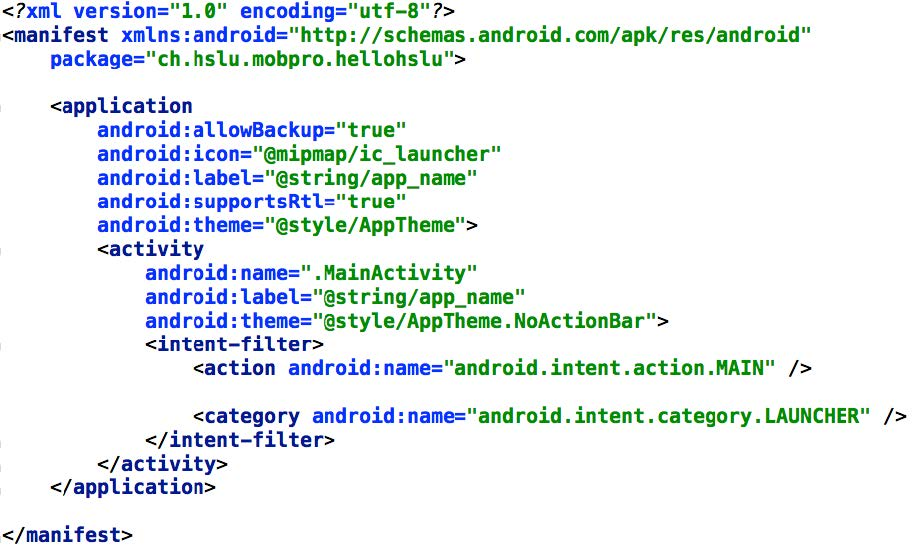
\includegraphics[width=12cm]{img/manifestxml.jpg}
	\caption{Beispiel eines Android-Manifests}
	\label{fig:manifestxml}
\end{figure}
\subsection{Activities \& Aufruf mit Intents}
Zwischen Komponenten herrscht das Prinzip der losen Kopplung:
\begin{itemize}
	\item Komponenten rufen andere Komponenten über Intents (= Nachrichten) auf
	\item Offene Kommunikation: Sender weiss nicht ob Empfänger existiert
	\item Parameterübergabe als Strings (untypisiert)
	\item Parameter: von Empfänger geprüft, geparst \& interpretiert (oder ignoriert)
	\item Keine expliziten Abhängigkeiten $\rightarrow$ Robuste Systemarchitektur
\end{itemize}
\newpage
\begin{figure}[htb!]
	\centering
	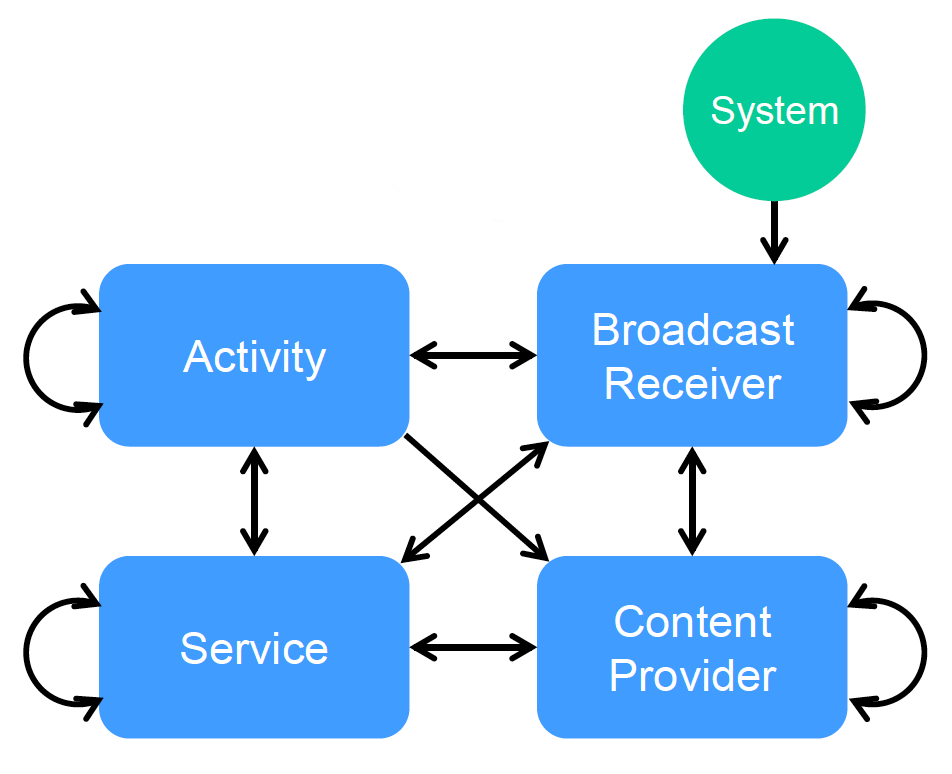
\includegraphics[width=7.5cm]{img/intents_comm.png}
	\caption{Kommunikation zwischen Komponenten mit Intents}
	\label{fig:intents_comm}	
\end{figure}
\noindent
Intents werden benutzt, um Komponenten zu benachrichtigen oder um Kontrolle zu übergeben. Es gibt folgende zwei Arten von Intents:
\begin{description}
	\item[Explizite Intents] adressieren eine Komponente direkt
	\item[Implizite Intents] beschreiben einen geeigneten Empfänger
\end{description}
\textbf{WICHTIG:} Activities müssen immer im Manifest deklariert werden, da sie sonst nicht als "public" gelten und eine Exception schmeissen. Das geht auch ganz einfach folgendermassen im Manifest unter "application":
\begin{lstlisting}
<activity android:name=".Sender" />
<activity android:name=".Receiver" />
\end{lstlisting}
\subsubsection{Beispielaufruf Expliziter Intent}
\textbf{Sender Activity:}
\begin{lstlisting}
public void onClickSendBtn(final View btn) {
	Intent intent = new Intent(this, Receiver.class); 
	// Receiver.class ist hier der explizite Empfaenger
	intent.putExtra("msg", "Hello World!");
	startActivity(intent);
}
\end{lstlisting}
\textbf{Receiver Activity:}
\begin{lstlisting}
public void onCreate(Bundle savedInstanceState) {
	// ...
	Intent intent = getIntent();
	String msg = intent.getExtras().getString("msg");
	displayMessage(msg);
}
\end{lstlisting}
\newpage
\subsubsection{Beispielaufruf Impliziter Intent}
\textbf{Sender Activity:}
\begin{lstlisting}
Intent browserCall = new Intent();
browserCall.setAction(Intent.ACTION_VIEW);
browserCall.setData(Uri.parse("http://www.hslu.ch"));
startActivity(browserCall);	
\end{lstlisting}
\textit{ACTION\_VIEW} ist hierbei kein expliziter Empfängertyp, sondern nur eine gewünschte Aktion. Die mitgege\-bene URL wird auch ein \textit{Call Parameter} genannt. Gesucht ist in diesem Fall eine Komponente, welche eine URL anzeigen/verwenden kann.\\
\subsection{Activities \& Subactivities}
\textbf{Activity Back Stack:} Activities liegen aufeinander wie ein Stapel Karten, neuste Activity zuoberst und in der Regel ist nur diese sichtbar (Durch Transparenz sind hier Ausnahmen möglich).
Durch "back" oder "finish" wird die oberste Karte entfernt und man kehrt zur zweitletzten Activity zurück. Mehrere Instanzen derselben Activity wären mehrere solche Karten, das Verhalten kann jedoch konfiguriert werden (z.Bsp. maximal eine Instant, mehrere Activities öffnen, etc.)\\
\textbf{(Sub-)Activities und Rückgabewerte:} Eine Activity kann Rückgabewerte einer anderen (Sub-)Activity erhalten.
\begin{lstlisting}
// 1. Aufruf der SubActivity mit
startActivityForResult(intent, requestId)

// 2. SubActivity setzt am Ende Resultat mit
setResult(resultCode, intent) // intent als Wrapper fuer Rueckgabewerte

// 3. SubActiity beendet sich mit
finish()

// 4. Nach Beendung der SubActivity wird folgendes im Aufrufer aufgerufen:
onActivityResult(requestId, resultCode, intent)
// resultCode: RESULT_OK, RESULT_CANCELLED
\end{lstlisting}
\subsection{Lebenszyklus \& Zustände von Applikationen/Activities}
Das System kann Applikationen bei knappem Speicher ohne Vorwarnung terminieren (nur Activities im Hintergrund, dies geschieht unbemerkt vom User, die App wird bei Zurücknavigation wiederhergestellt). Eine Applikation kann ihren Lebenszyklus demnach nicht kontrollieren und muss in der Lage sein, ihren Zustand speichern und wieder laden zu können. Applikationen durchlaufen mehrere Zustände in ihrem Lebenszyklus, Zustandsübergänge rufen Callback-Methoden auf (welche von uns überschrieben werden können.\\

\noindent
\textbf{Activity-Zustände:}
\begin{table} [h!]
	\begin{tabular}{ c | p{10cm} }
		\textbf{Zustand} & \textbf{Beschreibung} \\ \hline
		\textbf{Running} & Die Activity ist im Vordergrund auf dem Bildschirm (zuoberst auf dem Activity-Stack für die aktuelle Aufgabe). \\ \hline
		\textbf{Paused} & Die Activity hat den Fokus verloren, ist aber immer noch sichtbar für den Benutzer. \\ \hline
		\textbf{Stopped} & Die Activity ist komplett verdeckt von einer andern Activity. Der Zustand der Activity bleibt jedoch erhalten.
	\end{tabular}
\end{table}
\newpage
\subsubsection{Lifecycle einer Applikation}
\begin{figure}[h!]
	\centering
	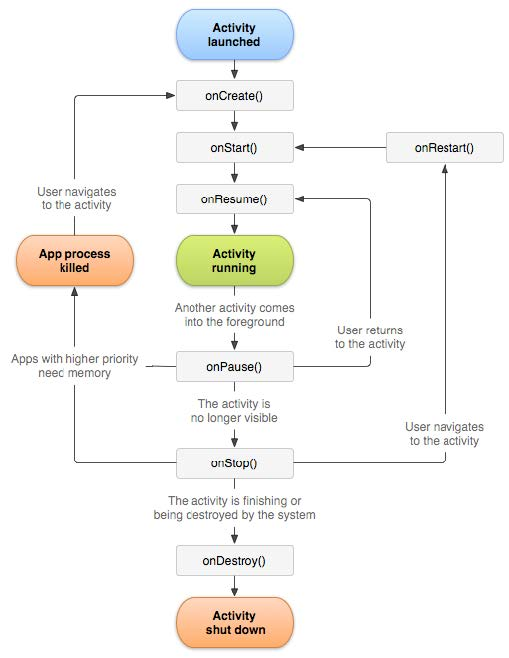
\includegraphics[width=13cm]{img/lifecycle.jpg}
	\caption{Lifecycle einer Applikation}
	\label{fig:lifecycle}
\end{figure}
\begin{figure}[h!]
	\centering
	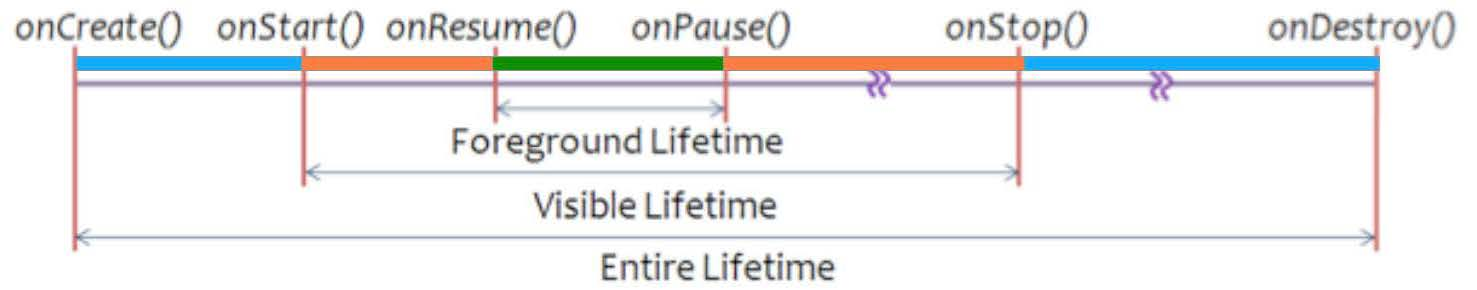
\includegraphics[width=11cm]{img/lifetime.jpg}
	\caption{Lebenszeiten der einzelnen App-Zustände}
	\label{fig:lifetime}
\end{figure}
\newpage
\subsection{Charakterisierung einer Activity}
\begin{itemize}
	\item Muss im Manifest deklariert werden
	\item GUI-Controller
	\begin{itemize}
		\item Repräsentiert eine Applikations-/Bildschirmseite
		\item Definiert Seitenlayout und GUI-Komponenten
		\item Kann aus Fragmenten ( = "Sub-Activities") aufgebaut sein
		\item Reagiert auf Benutzereingaben
		\item Beinhaltet Applikationslogik für dargestellte Seite
	\end{itemize}
\end{itemize}
\textbf{Beispiel einer Activity:}
\begin{lstlisting}
public class Demo extends Activity {
	// Called when the Activity is first created
	public void onCreate(Bundle savedInstanceState) {
		super.onCreate(savedInstanceState);
		setContentView(R.layout.main); // Definiert Layout und UI
	} 
}	
\end{lstlisting}
\subsubsection{Zustandsänderung - Hook-Methoden}
Das System benachrichtigt Activities durch Aufruf einer der folgenden Methoden der Klasse \textit{Activity}:
\begin{itemize}
	\item void onCreate(Bundle savedInstanceState)
	\item void onStart() / void onRestart()
	\item void onResume()
	\item void onPause() $\rightarrow$ \textit{bspw. Animation stoppen}
	\item void onStop()
	\item void onDestroy() $\rightarrow$ \textit{bspw. Ressourcen freigeben}
\end{itemize}
Durch das Überschreiben dieser Methoden können wir uns in den Lebenszyklus einklinken. Immer \textbf{super()} aufrufen, sonst wirft es eine Exception.
\newpage
\subsection{Android - Hinter den Kulissen}
\begin{figure}[h!]
	\centering
	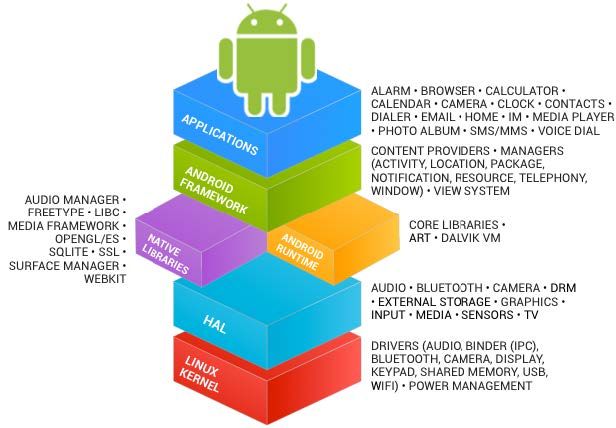
\includegraphics[width=11cm]{img/androidstack.jpg}
	\caption{Der Android-Stack}
	\label{fig:androstack}
\end{figure}
\begin{itemize}
	\item \textbf{Linux-Kernel:} OS, FS, Security, Drivers, ...
	\item \textbf{HAL (Hardware Abstraction Layer):} Camera-, Sensor-, ... Abstraktion
	\item \textbf{ART} (Android Runtime)
	\begin{itemize}
		\item Jede App in eigenem Prozess
		\item Optimiert für mehrere JVM auf low-memory Geräten
		\item Eigenes Bytecode-Format (Crosscompiling)
		\item JIT und AOT Support
	\end{itemize}
	\item \textbf{Native C/C++ Libriaries:} Zugriff via Android NDK
	\item \textbf{Android Framework:} Android Java API
	\item \textbf{Applications:} System- und eigene Apps
\end{itemize}
\newpage
\subsubsection{Android-Security-Konzept}
\textbf{Sandbox-Konzept:} 
\begin{itemize}
	\item Jede laufende Android-Anwendung hat seinen eigenen Prozess, Benutzer, ART-Instanz, Heap und Dateisystembereich $\rightarrow$ jedes App hat eigenen Linux-User
	\item Das Berechtigungssystem von Linux ist Benutzer-basiert, es betrifft deshalb sowohl den Speicherzugriff wie auch das Dateisystem. 
	\item Anwendungen signieren: erschwert Code-Manipulationen und erlaubt das Teilen einer Sandbox bei gleicher sharedUser-ID
	\item Berechtigungen werden im Manifest deklariert, kontrollierte Öffnung der Sandbox-Restriktionen
\end{itemize}
\begin{figure}[htb!]
	\centering
	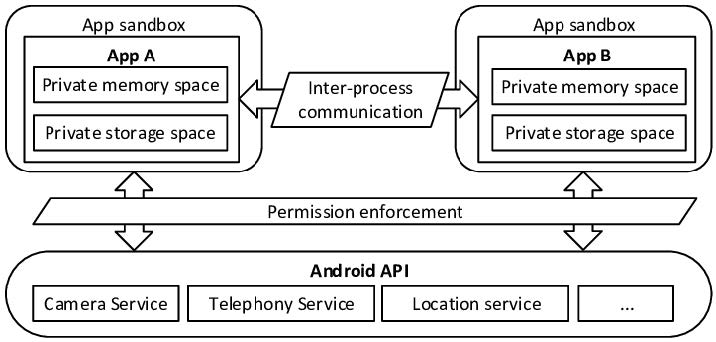
\includegraphics[width=12cm]{img/securitymodel.jpg}
	\caption{Android Security-Modell}
	\label{fig:secumodel}
\end{figure}

\newpage
\section{Android 2 - Benutzerschnittstellen}

\subsection{GUI einer Activity}

GUI wird als XML definiert, der Name resultiert in einer Konstante: \textit{\textbf{R}.layout.xxx}. Diese wird im \textit{onCreate()} einer Activity mit \textit{setContentView()} angegeben.

\begin{figure}[htb!]
	\centering
	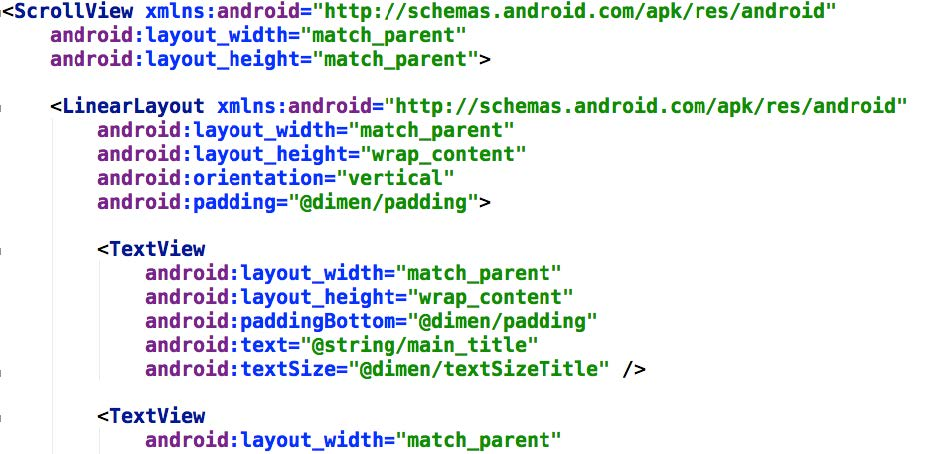
\includegraphics[width=10cm]{img/gui_xml_example.jpg}
	\caption{Beispiel eines XML für ein Layout}
	\label{fig:guixmlexamp}
\end{figure}
\noindent
Je nach Layout müssen die Elemente unterschiedlich konfiguriert werden, was bei der Arbeit mit dem Layout-Editor nicht offensichtlich, aber trotzdem gut zu wissen ist. \\
Ein Android-UI ist hierarchisch aufgebaut und besteht aus \textbf{ViewGroups} (Cointainer für Views oder weitere ViewGroups, angeordnet durch Layout) und \textbf{Views} (Widgets). Sollte auf unterschiedlichen Bildschirmgrössen gleich aussehen (Elemente deshalb \textbf{relativ} und nicht absolut positionieren)

\begin{figure}[htb!]
	\centering
	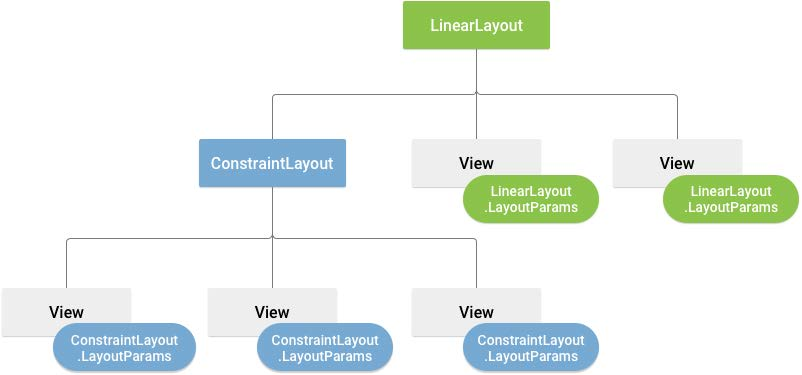
\includegraphics[width=10cm]{img/xml_layouts.jpg}
	\caption{Layout-Varianten bei Android}
	\label{fig:xmllayouts}
\end{figure}
\noindent
Schachtelung möglich, aber nicht effizient, wenn möglich immer das Constraint-Layout verwenden. Layouts spezifiziert man auf zwei verschiedene Arten:
\begin{itemize}
	\item \textbf{Statisch / Deklarativ (XML)}
	\item \textit{Grundsätzlich in MOBPRO verwendet, bietet viele Vorteile (Deklarativ, weniger umständlich als Code, Struktur eminent, Umformungen ohne Rekompilierung möglich...)}
		\begin{itemize}
			\item Deklarative Beschreibung des GUI als Komponentenbaum
			\item XML-Datei unter \textit{res/layout}
			\item Referenzen auf Bilder/Texte/etc.
			\item Typischerweise ein XML pro Activity
		\end{itemize}
	\item \textbf{Dynamisch (in Java)}
	\item \textit{Jedes XML hat eine korrespondierende Java-Klasse, XML $\rightarrow$ Java = Inflating}
		\begin{itemize}
			\item Aufbau und Definition des GUI im Java-Code
			\item Normalerweise nicht nötig: die meisten GUIs haben fixe Struktur
			\item Änderung von Eigenschaften während Laufzeit ist normal (Bsp. Visibility, Ausblenden einer View, wenn nicht benötigt)
		\end{itemize}
\end{itemize}
\newpage
\subsection{XML-Layout}
\begin{itemize}
	\item Jedes Layout ist ein eigenes XML-File
	\begin{itemize}
		\item Root-Element = View oder ViewGroup
		\item Kann Standard- oder eigene View-Klassen enthalten
	\end{itemize}
	\item XML können mit Inflater "aufgeblasen" bzw. instanziiert werden, damit eigene wiederverwendbare Komponenten/Templates/Prototypen erzeugt werden können
	\item Innere Elemente können unterhalb eines Parents via View-ID referenziert werden (\textit{findViewById()})
	\item Debugging mit dem Layout-Inspector	
\end{itemize}

\subsubsection{Constraint-Layout}

\begin{multicols}{2}
\begin{itemize}
	\item Erstellung von komplexen Layouts, ohne zu schachteln
	\item Elemente werden relativ mit Bedingungen platziert
	\begin{itemize}
		\item zu anderen Elementen
		\item zum Parent-Container
		\item Element-Chains (spread/pack)
	\end{itemize}
	\item Layout-Hilfen (Hilfslinien, Barriers)
\end{itemize}
\columnbreak
\begin{minipage}[c]{\columnwidth}
	\centering
	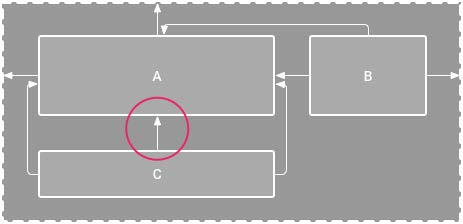
\includegraphics[width=0.7\linewidth]{img/constraintlayout.jpg}
	\captionof{figure}{Constraint Layout}
\end{minipage}
\end{multicols}

\subsubsection{LinearLayout}

\begin{multicols}{2}
\begin{itemize}
	\item Reiht Elemente neben-/untereinander auf
	\begin{itemize}
		\item kann geschachtelt werden, um Zeilen/Spalten zu formen (nicht zu tief, sonst schlechte Performanz
	\end{itemize}
	\item Eigenschaften:\\
	 \textit{(orientation, gravity, weigthSum, etc.)}
	\item Layout-Parameter für Children
	\begin{itemize}
		\item layout\_width, layout\_height
		\item layout\_margin...
		\item layout\_weight, layout\_gravity
	\end{itemize}
\end{itemize}
\columnbreak
\begin{minipage}[c]{\columnwidth}
	\centering
	
\includegraphics[width=0.5\linewidth]{img/linearlayout.jpg}
	\captionof{figure}{LinearLayout}
\end{minipage}
\end{multicols}

\paragraph{Warum nutzt man trotzdem noch LinearLayout?}
\begin{itemize}
	\item Nach wie vor einfachste Lösung für Button- oder Action-Bars ("flow semantik") und einfache Screens
	\item Kaum Konfiguration nötig, robust
	\item Für scrollbare Listen mit dynamischer Anzahl Elemente besser \textit{ListView} verwenden (siehe Adapter-Views)
	\item Einsatz mit Bedacht durchaus sinnvoll
\end{itemize}
\vspace{1em}
\noindent
Es gibt noch die \textbf{ScrollView}, deren Nutzung vertikales Scrollen bei zu grossen Layouts erlaubt, sie kann jedoch \underline{nur ein Kind} haben und enthält typischerweise das Top-Level-Layout einer Bildschirmseite.

\paragraph{Pixalangaben}
\textit{(Typischerweise werden Angaben in dp verwendet, ausser sp bei Schriftgrössen.)}
\begin{itemize}
	\item \textbf{dp - density-independent:} \\ Passen sich der physischen Dichte des Screens an, dp passen sich gegenüber den realen Dimensionen eines Screens und dessen Verhältnisse an.
	\item \textbf{sp - scale-independent:} \\Ähnlich der dp-Einheit, passt sich jedoch der Schriftskalierung des Nutzers an.
	\item \textbf{px - Pixels:} \\Passen sich der Anzahl Pixel eines Bildschirms an, deren Nutzung wird nicht empfohlen.
\end{itemize}

\newpage

\subsection{Ressourcen, Konfigurationen und Internationalisierung}
\textbf{Ressourcen} sind alle Nicht-Java-Teile einer Applikation und sind im \textit{/res}-Verzeichnis abgelegt, sogennante ausgelagerte Konstanten-Definitionen. Sie werden im Layout und Java-Code über die \textbf{\textit{automatisch generierte R-Klasse}} mit ID-Konstanten (int) referenziert. Kontextabhängige Ressourcen sind möglich z.Bsp. für Sprache, Gerätetyp, Orientierung, ...\\
\textbf{Beispiele}: Strings, Styles, Colors, Dimensionen, Bilder (drawables), Layouts (portrait, landscape), Array-Werte (z.Bsp. für Spinner) und Menü-Items\\

\begin{figure}[htb!]
	\centering
	\begin{subfigure}{0.5\textwidth}
		\centering
		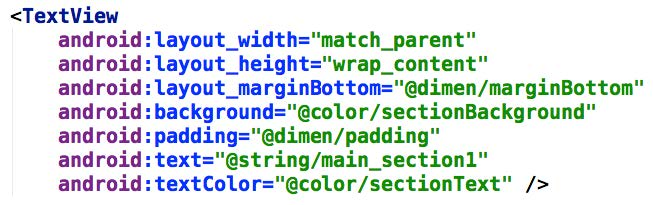
\includegraphics[width=0.8\linewidth]{img/references_xml.jpg}
		\caption{Referenz in XML mit @}
	\end{subfigure}%
	\begin{subfigure}{0.5\textwidth}
		\centering
		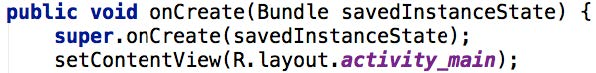
\includegraphics[width=0.8\linewidth]{img/references_code.jpg}
		\caption{Referenz in Code über \texttt{R}-Klasse, diese wird beim Build automatisch generiert}
	\end{subfigure}
\end{figure}
\noindent
Für verschiedene Systemkonfigurationen benötigt es unterschiedliche Ausprägungen einer Ressource, beispielsweise:
\begin{itemize}
	\item \textbf{Internationalisierung}: komplette/teilweise Übersetzung, für diese werden unterschiedliche Ordner je nach Land/Sprache und seperate .xml angelegt
	\item \textbf{Auflösungsklassen}: \texttt{ldpi} (~120dpi), \texttt{mdpi} (~160dpi), \texttt{hdpi} (~240dpi), \texttt{xhdpi} (~320dpi) 
	\item \textbf{Orientierung} des Displays: landscape / portrait
	\item Verschiedene \textbf{HW-Modelle}: HTC, Samsung, Sony, LG, ...
\end{itemize}
Default-Verzeichnisse sind innerhalb von \texttt{res/} angelegt: drawable, layout, menu, values, ...\\
Bei spezifischen Konfigurationen werden meist Kopien der Default-Verzeichnisse/Ordner mit einem Suffix angelegt, bspw. \texttt{res/strings-de-rCH}, in welchen dann die Ressourcen (XML) erneut angelegt werden.
\begin{figure}[htb!]
	\centering
	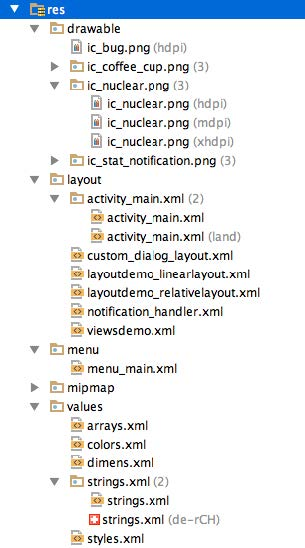
\includegraphics[width=0.3\linewidth]{img/ressources.jpg}
	\caption{Beispiel der Default-Ressourcen}
\end{figure}

\newpage
\subsection{UI-Event-Handling}
\begin{itemize}
	\item Jedes View-Element hat eine entsprechende Java-Klasse (auch View-Groups!) \\$\rightarrow$ Layout könnte auch dynamisch in Java programmiert werden
	\item APIs der einzelnen View-Klassen sind \href{http://developer.android.com/reference/android/widget/package-summary.html}{hier} oder unter "Nützliche Links" genauer beschrieben
\end{itemize}
\begin{figure}[htb!]
	\centering
	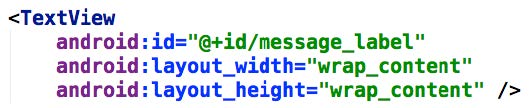
\includegraphics[width=0.5\linewidth]{img/layout_id.jpg}
	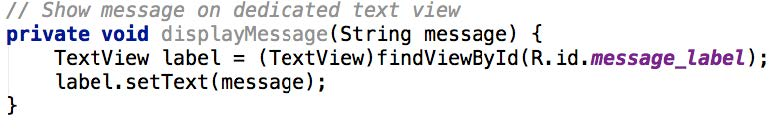
\includegraphics[width=0.5\linewidth]{img/reference_code.jpg}
	\caption{ID im Layout erfassen und Referenz im Code}
\end{figure}

\subsubsection{GUI-Events}
\begin{itemize}
	\item \textbf{Observer/Listener}: einen Listener für ein entsprechendes Event bei der View registrieren, bspw. bei \texttt{Button myButton}:\\
	\texttt{myButton.setOnClickListener(listener)}
	\item verschiedenste Event- und Listener-Typen:\\
	\texttt{OnClickListener,  OnLongClickListener,  OnKeyListener,  OnTouchListener,  OnDragListener, ...} 
	\\$\rightarrow$ \texttt{public static} Interfaces der Klasse \texttt{View}
\end{itemize}
\textbf{Ziel:} Auf Klick-Event eines Buttons reagieren
\begin{itemize}
	\item Button muss eine ID haben im layout.xml
	\item Registrierungs eines Listeners an die View (Button) im Code:
\end{itemize}
\begin{lstlisting}
Button button = (Button) findViewById(R.id.question_button_done);
button.setOnClickListener(new OnClickListener() {
	@Override
	public void onClick(View v) {
		// handler code
		buttonClicked();
	}
});
\end{lstlisting}
\textbf{onClick-Event-Registrierung in XML}
\begin{figure}[htb!]
	\centering
	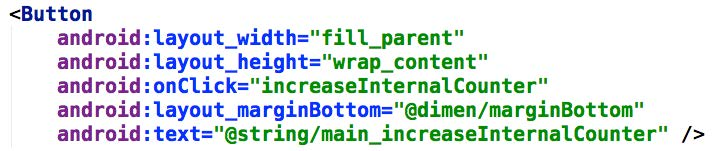
\includegraphics[width=0.6\linewidth]{img/onclick.jpg}
	\caption{Definition onClick-Handler im Layout $\rightarrow$ so nur für OnClick-Events}
\end{figure}
\begin{lstlisting}
// Implementierung OnClick-Handler-Methode in der Activity
public void increaseInternalCounter(View button){
	// ... handler code ...
}
\end{lstlisting}

\newpage

\subsubsection{Exkurs: Data Binding}

\begin{figure}[htb!]
	\centering
	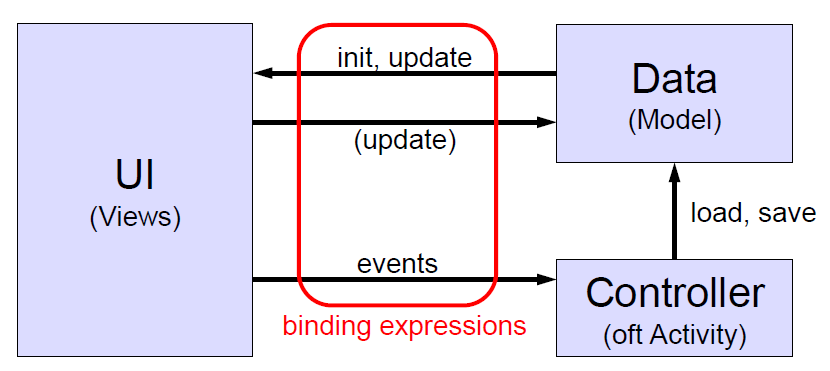
\includegraphics[width=0.5\textwidth]{img/data_binding_model.png}
	\caption{Modell für Data Binding}
\end{figure}
\noindent
\textbf{Data Binding:} separiert UI und Daten, synchronisiert UI mit Daten (1-, resp. 2-way-binding), verwendet «binding expressions» mit @{..} Syntax im Layout-File, um View-Attribute zu initialisieren. Anbei ein Beispiel (auskommentiert):

\begin{lstlisting}
<?xml version="1.0" encoding="utf-8"?> 
<layout xmlns:android="http://schemas.android.com/apk/res/android"> 
	<data> 
		<variable name="model" type="org.example.MyModel"/> 
	</data>  // Definition der Layout-Variablen
	<LinearLayout ...> 
		<Button 
			android:id="@+id/button" 
			...
			android:enabled="@{model.user.role == `admin`}" 
			android:text="@{model.buttonText}" // Data Binding (1-way)
			...
			android:onClick="@{() -> model.increaseClickCount()}" /> // Event Binding
		<EditText 
			android:id="@+id/input"
			...
			android:text="@={model.inputText}"/> // Data Binding (2-way)
	</LinearLayout> 
</layout>

protected void onCreate(Bundle savedInstanceState) { 
	super.onCreate(savedInstanceState); 
	ActivityMainBinding binding = DataBindingUtil.setContentView(...); 
	model = new MainModel();
	model.load(); 
	binding.setModel(model);
	// Binden der Layout-Daten auf effektive Daten
	// z.B. ViewModel mit Observables
}
\end{lstlisting}
\newpage

\subsection{Options-Menü}

\begin{itemize}
	\item Android-Apps können oben rechts ein Menü mit Optionen anbieten
	\item Erzeugung durch Aufruf \textit{Hook} in der Activity-Klasse:\\
	\texttt{onCreateOptionsMenu(Menu menu)}
	\begin{itemize}
		\item Hier kann ein Menü mit Einträgen bestückt werden
		\item \texttt{MenuInflater} + XML benutzen oder Java oder beides
	\end{itemize}
	\item Beim Klick auf Eintrag Aufruf eines anderen Hooks:\\
	\texttt{onOptionsItemSelected(MenuItem item)}
\end{itemize}
\noindent
Für ein Options-Menü muss eine .xml-Datei (Bsp. main\_menu.xml) im Ordner \texttt{res/menu} angelegt werden. Danach werden Informationen folgendermassen eingetragen:
\begin{figure}[htb!]
	\begin{subfigure}{0.5\textwidth}
		\centering
		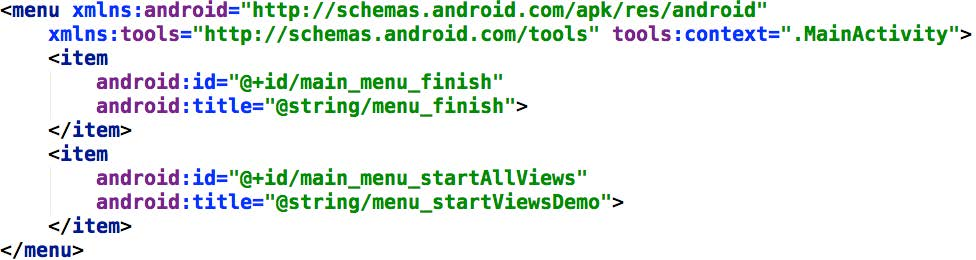
\includegraphics[width=\linewidth]{img/menu_example.jpg}
		\caption{Menü und Items in XML definieren}
	\end{subfigure}
	\begin{subfigure}{0.5\textwidth}
		\centering
		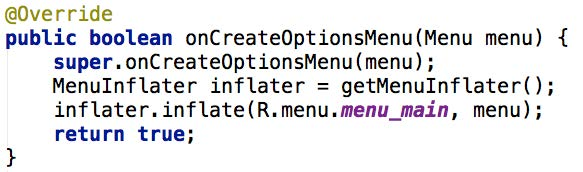
\includegraphics[width=\linewidth]{img/menuinflater.jpg}
		\caption{Menü mit \texttt{MenuInflater} aufblasen}
	\end{subfigure}
\end{figure}

Um bspw. einen String in einem Menüpunkt einzufügen, gibt es drei verschiedene Möglichkeiten:
\begin{figure}[htb!]
	\centering
	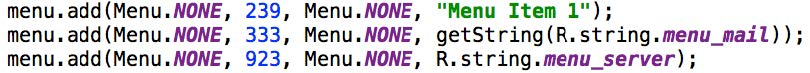
\includegraphics[width=.8\textwidth]{img/menu_string.jpg}
	\caption{Möglichkeiten zum Einlesen eines Strings}
\end{figure}
\begin{figure}[htb!]
	\centering
	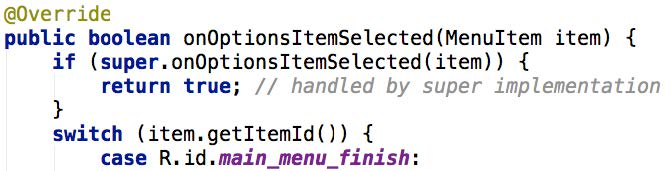
\includegraphics[width=.7\textwidth]{img/menu_selektierung.jpg}
	\caption{Event-Handling: Selektierung}
\end{figure}

\newpage

\subsection{Adapter-Views}
\emph{Behandelt wird hier nur das synchrone Laden von kleinen/schnellen Datenquellen, für asynchrones Laden von langsamen/grossen Datenquellen konsultiere Doku über \textbf{Loaders}.}
\begin{figure}[htb!]
	\centering
	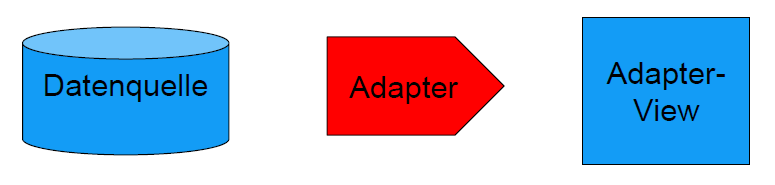
\includegraphics[width=.8\textwidth]{img/adapter.png}
	\caption{Aufgabe des Adapters}
\end{figure}
\begin{itemize}
	\item Adapter $\rightarrow$ Verbindung zwischen Datenquelle und GUI
	\item Zapft \textit{Datenquelle} an und beliefert \textit{AdapterView}
	\item Erzeugt (Sub-)Views pro gefundenes Datenelement
	\item Transformiert Daten ggf. in benötigtes Zielformat
	\item Datenquellen:\\
	String-Array, String-Liste, Bilder, Datenbank, ...
\end{itemize}

\vspace{3em}

\begin{figure}[htb!]
	\centering
	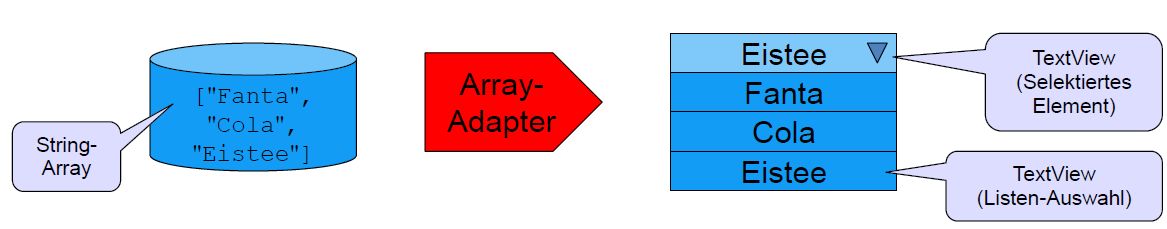
\includegraphics[width=.8\textwidth]{img/adapter_string.png}
	\caption{Beispiel eines ArrayAdapter}
\end{figure}
\begin{itemize}
	\item Bindet irgend ein Array oder Liste mit beliebig getypeten Elementen an irgend eine AdapterView
	\item Für jedes Daten-Element wird eine SubView erzeugt
	\item \textbf{Default}: Erstellt \texttt{TextView} mit \texttt{element.toString()}-Wert
\end{itemize}
\begin{figure}[htb!]
	\centering
	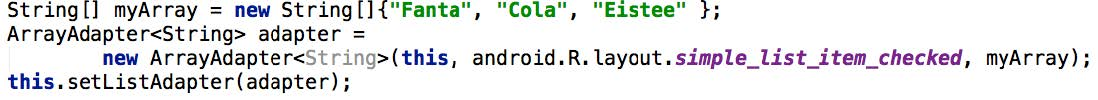
\includegraphics[width=.8\textwidth]{img/adapterview_example.jpg}
	\caption{Beispiel einer AdapterView}
\end{figure}

\subsubsection{AdapterViews \& ListActivity}

\begin{itemize}
	\item \textbf{AdapterViews}: spezielle View-Klassen
		\begin{itemize}
			\item Sind für Zusammenarbeit mit Adaptern optimiert \\
			(Bsp.\texttt{ListView, GridView, Gallery, Spinner, Stack,...})
			\item Füllen Teile von sich mit von Adaptern erzeugten Views
			\item Leiten ab von \texttt{android.widget.AdapterView<T extends android.widget.Adapter>}
		\end{itemize}
	\item Spezielle Activity: \textbf{ListActivity}
		\begin{itemize}
			\item Vordefiniertes Layout (enthält eine \texttt{ListView}, kein XML nötig)
			\item Vordefinierte Callbacks (bei Auswahl einer List-Entry)
			\item Bietet Zugriff auf aktuelle Selektion / Datenposition
		\end{itemize}
\end{itemize}

\newpage

\subsubsection{android.widget.Spinner}

\begin{itemize}
	\item ComboBox oder DropDown-List genannt (weitere Alternative: AutoCompleteTextView)
	\item Zeigt ein ausgewähltes Element, bei Klick erscheint ein Auswahlmenü
	\item 2 Varianten, um Daten auf Spinner zu setzen:
		\begin{itemize}
			\item Im Code mit Adapter:\\
			\texttt{spinner.setAdapter(myAdapter)}
			\item Im XML mit Angabe einer String-Array-ID:\\
			\texttt{android:entries="@array/spinnerValues"}
		\end{itemize}
	\item Listener setzen für Behandlung der Auswahl:\\
	\texttt{spinner.setOnItemSelectedListener(...)}
\end{itemize}
\vspace{2em}
\begin{figure}[htb!]
	\centering
	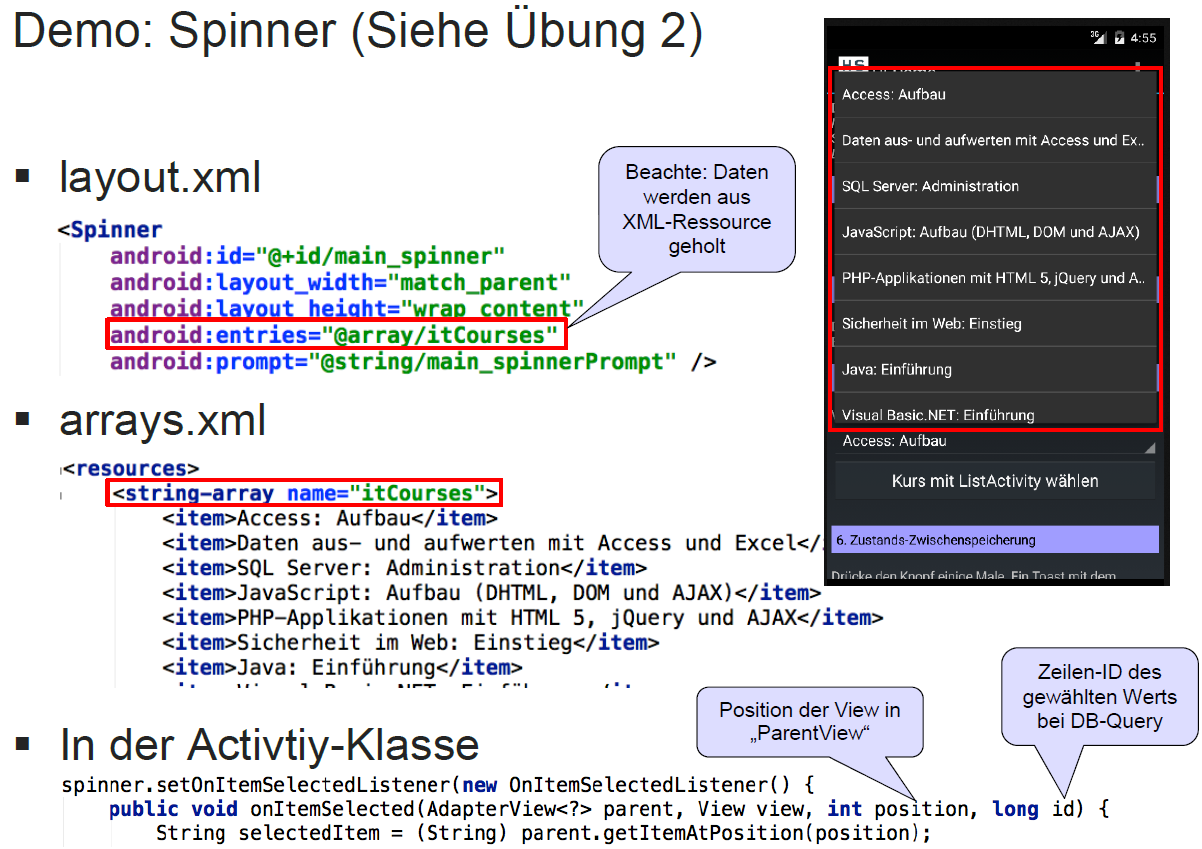
\includegraphics[width=\textwidth]{img/spinner_demo.png}
	\caption{Übungs-Demo aus der Vorlesung SW02 - Spinner}
\end{figure}

\newpage

\subsubsection{android.widget.ListView}

\begin{itemize}
	\item Liste von Views/Items, die zur Auswahl stehen
	\item Braucht viel Platz! Meist wird ihr der ganze Bildschirm zugeteilt
	\item i.d.R. zusammen mit \texttt{ListActivity} verwendet, Verwendung:
		\begin{enumerate}
			\item Navigiere zu eigener ListActivity
			\item Auswahl $\rightarrow$ Resultat setzen $\rightarrow$ finish
			\item Auswertung des Rückgabewert im Caller
		\end{enumerate}
	\item Konzeptionell identisch zum Spinner, jedoch andere Darstellung auf UI
		\begin{itemize}
			\item Verwendungsentscheid:
			\begin{itemize}
				\item Kurze Liste $\rightarrow$ Spinner
				\item (Sehr) lange Listen $\rightarrow$ ListView / ListActivity
				\item Kennt der User die möglichen Auswahlwerte $\rightarrow$ AutoCompleteTextView
			\end{itemize}
			\item Adapter- / Datendefinition grundsätzlich bei beiden gleich\\
			(d.h. im Code oder durch XML-Array)
			\item Auswahlmodus: \texttt{setChoiceMode(ListView.CHOICE\_MODE\_*} \\
			$\rightarrow$ Single- / Multiselection
		\end{itemize}
\end{itemize}

\subsubsection{android.app.ListActivity}

\begin{itemize}
	\item Spezielle Activity zur Darstellung einer ListView
	\item Vordefiniertes Layout (full-screen Liste)
		\begin{itemize}
			\item \texttt{setContentView(...)} muss nicht aufgerufen werden
			\item Aufruf i.d.R. mit \texttt{startActivityForResult(...)}
			\item Vordefinierte vererbte Konfigurationsmethoden
				\begin{itemize}
					\item \texttt{setListAdapter(adapter)} setzt Daten für die Liste
					\item \texttt{getListView()} erlaubt Zugriff auf ListView-Instanz\\
					\textit{(anstelle von findViewById(..) + Casten)}
				\end{itemize}
		\end{itemize}
	\item Callback bei der Auswahl
		\begin{itemize}
			\item \texttt{onListItemClick(parentView, view, position, id)}\\
			Wird bei Auswahl aufgerufen (muss in Subklasse überschrieben werden, keine Listener-Registrierung nötig)
		\end{itemize}
\end{itemize}

\begin{figure}[htb!]
	\centering
	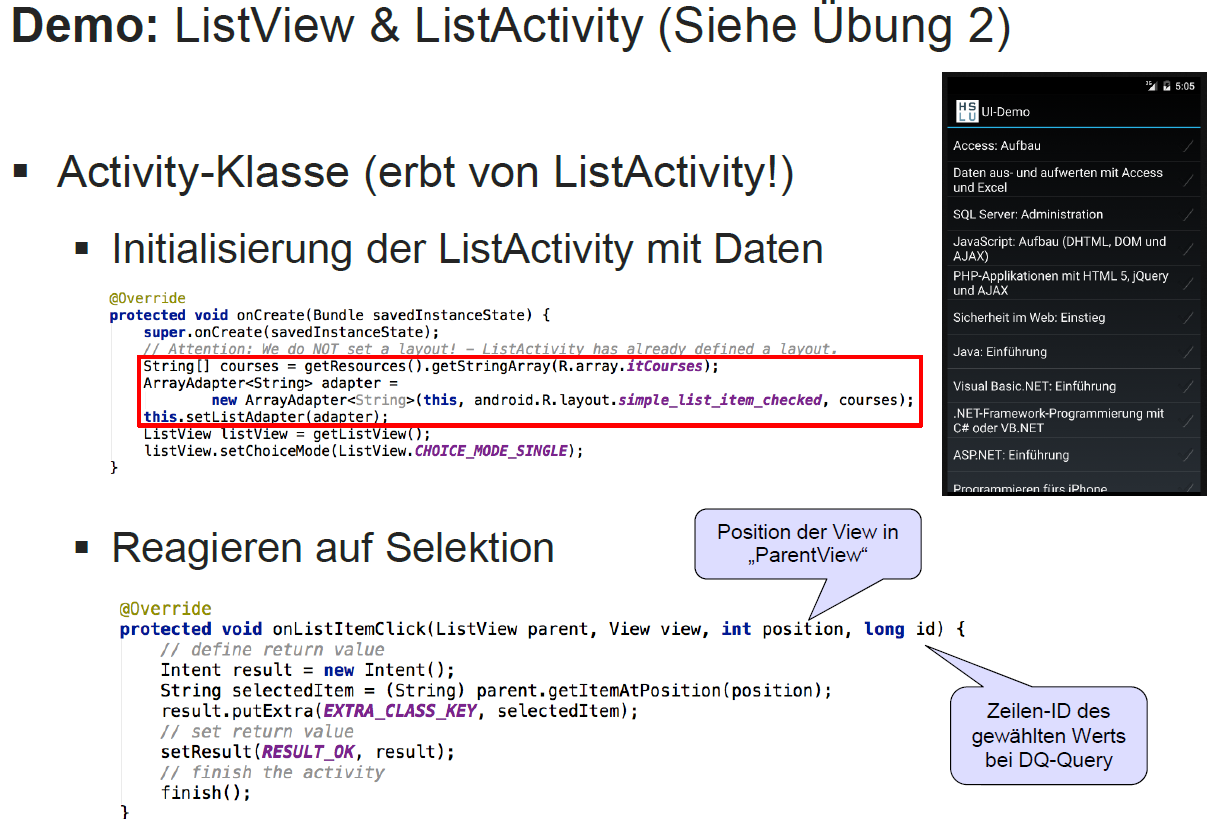
\includegraphics[width=.8\linewidth]{img/listview_demo.png}
	\caption{Übungs-Demo aus der Vorlesung SW02 - ListView / ListActivity}
\end{figure}

\newpage

\subsection{ViewModel - Konfigurationswechsel \& temporäre Datenspeicherung}

Bei jedem Konfigurationswechsel (z.B. Änderung Bildschirmorientation) wird die aktuelle Activity-Instanz zerstört und neu aufgebaut. Dabei besteht das Problem des \textbf{Zustandsverlusts}. Der Zustand alles Views mit einer ID (mit einigen Ausnahmen) wird automatisch gesichert und wiederhergestellt. Der \textbf{inhärente Zustand}, alles was nicht sichtbar und in Feldern gespeichert ist, geht jedoch verloren. Um entgegenzuwirken, kann ein \textbf{ViewModel} verwendet werden.

\begin{figure}[htb!]
	\centering
	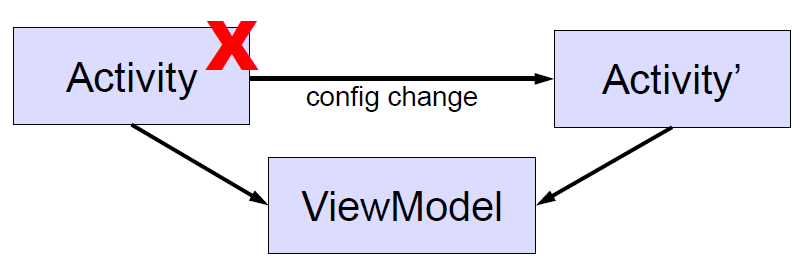
\includegraphics[width=.6\textwidth]{img/viewmodel}
	\caption{Position des ViewModels in der temp. Datenspeicherung}
\end{figure}

\begin{itemize}
	\item Kapselt UI-Daten so, dass diese bei einer Konfigurationsänderung einer Activity in-memory erhalten bleiben \textit{(Für den Fall eines App-Kills müssen Daten immer noch persistiert werden)}
	\item Lebensdauer mit der Activity gekoppelt
	\item Weniger Aufwand für Behandlung von Konfigurationsänderungen
\end{itemize}

\begin{figure}[htb!]
	\centering
	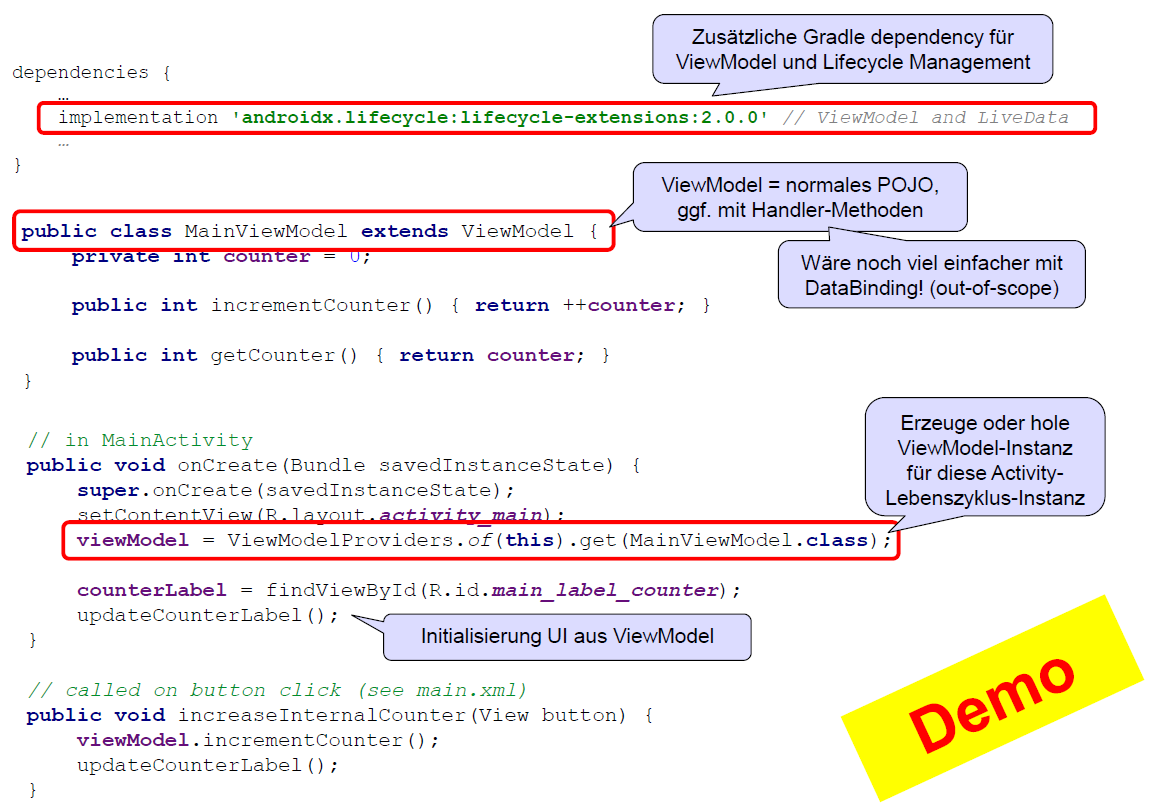
\includegraphics[width=\textwidth]{img/viewmodel_demo.png}
	\caption{Übungs-Demo aus der Vorlesung SW02 - ViewModel}
\end{figure}

\newpage

\subsection{Rückmeldungen an den Benutzer}

\subsubsection{Toast}

\begin{itemize}
	\item Kurze Rückmeldung (Popup) an den Benutzer, keine Interaktion möglich, verschwindet nach gewisser Zeit.
	\item Konfiguration: Text, Layout, Anzeigezeit (kurz/lang), Ort (gravity)
	\item Toasts mit eigenem Layout werden mit CustomToastView erstellt
\end{itemize}
\vspace{1em}
Beispielcode zur Erstellung von Toasts:

\begin{lstlisting}
// Default-Toast: Einzeiler
Toast.makeToast(getApplicationContext(), "Das ist..", Toast.LENGTH_LONG).show()
																						// LENGTH: Nur LONG oder SHORT
							// Kontext: meistens "this"
							
// Toast mit anderem Anzeigeort:
Context context = getApplicationContext();
Toast toast = Toast.makeText(context, "Toast links oben!", Toast.LENGTH_LONG);
toast.setGravity(Gravity.TOP|Gravity.START,0,0); // (x,y) Offset
toast.show()
\end{lstlisting}

\subsubsection{Alert-Dialog}

\begin{figure}[htb!]
	\centering
	
\includegraphics[width=.35\textwidth]{img/alert_dialog.jpg}
	\caption{Beispiel eines Alert-Dialogs}
\end{figure}

\begin{itemize}
	\item Fenster mit Interaktionsmöglichkeiten für den Benutzer
		\begin{itemize}
			\item Information / Eingabe von Daten
			\item Interaktion möglich
			\item Buttons: positive, neutral, negative
		\end{itemize}
	\item Vorteile
	\begin{itemize}
		\item Kaum Einschränken in punkto Darstellung
		\item Vorbereitet für die Anzeige von Daten
		\item Verschwindet erst, wenn sie vom Benutzer quittiert wurde
	\end{itemize}
	\item Konfiguration: Buttons, Titel, Icon, Nachricht\\
	Inhalt: Liste von Items oder eigene View
\end{itemize}

\newpage

\begin{itemize}
	\item Vorgehen beim Erstellen eines Alert-Dialog mit Builder-Muster
	\begin{enumerate}
		\item Builder erstellen: \texttt{new AlertBuilder.Builder(this)}
		\item Builder konfigurieren: \\
		\texttt{setXXX} + Registrierung von \texttt{ClickListeners}
		\item Dialog erstellen: \texttt{Dialog dialog = builder.create()}
		\item Dialog anzeigen: \texttt{dialog.show()}
	\end{enumerate}
	\item Anzeige von Dialogen ist \textbf{immer asynchron!}\\
	Bei \texttt{show()} wird nicht gewartet, kein Rückgabewert\\
	$\rightarrow$ Behandlung von Benutzerselektion mit Listener
\end{itemize}

\begin{figure}[htb!]
	\centering
	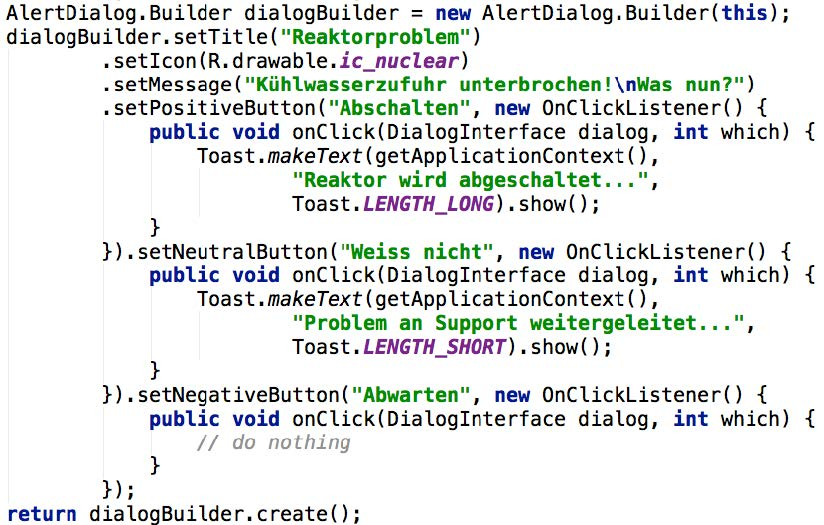
\includegraphics[width=.9\textwidth]{img/alertdialog.jpg}
	\caption{Beispiel eines AlertDialog aus Vorlesung}
\end{figure}

\newpage

\begin{figure}[htb!]
	\centering
	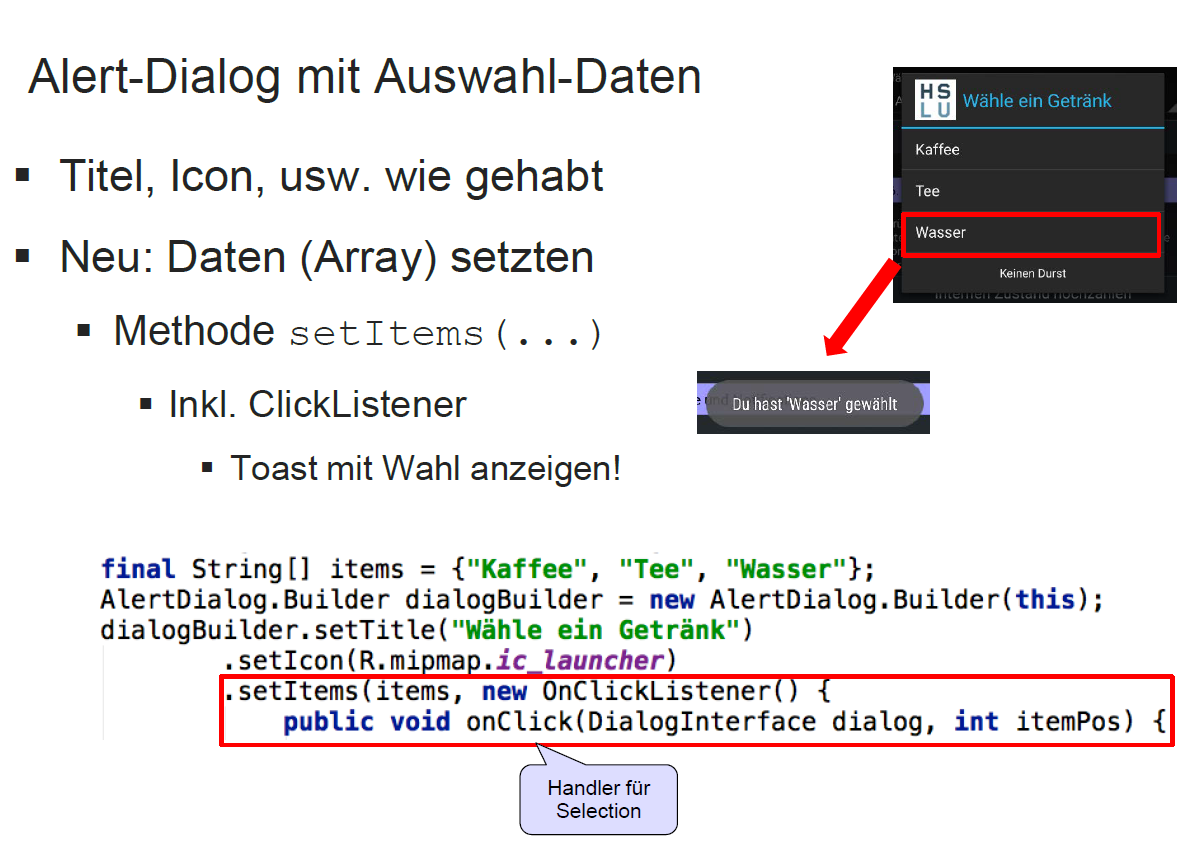
\includegraphics[width=\textwidth]{img/alertdialog_daten.png}
	\caption{Beispiel mit Auswahl-Daten}
\end{figure}
\begin{figure}[htb!]
	\centering
	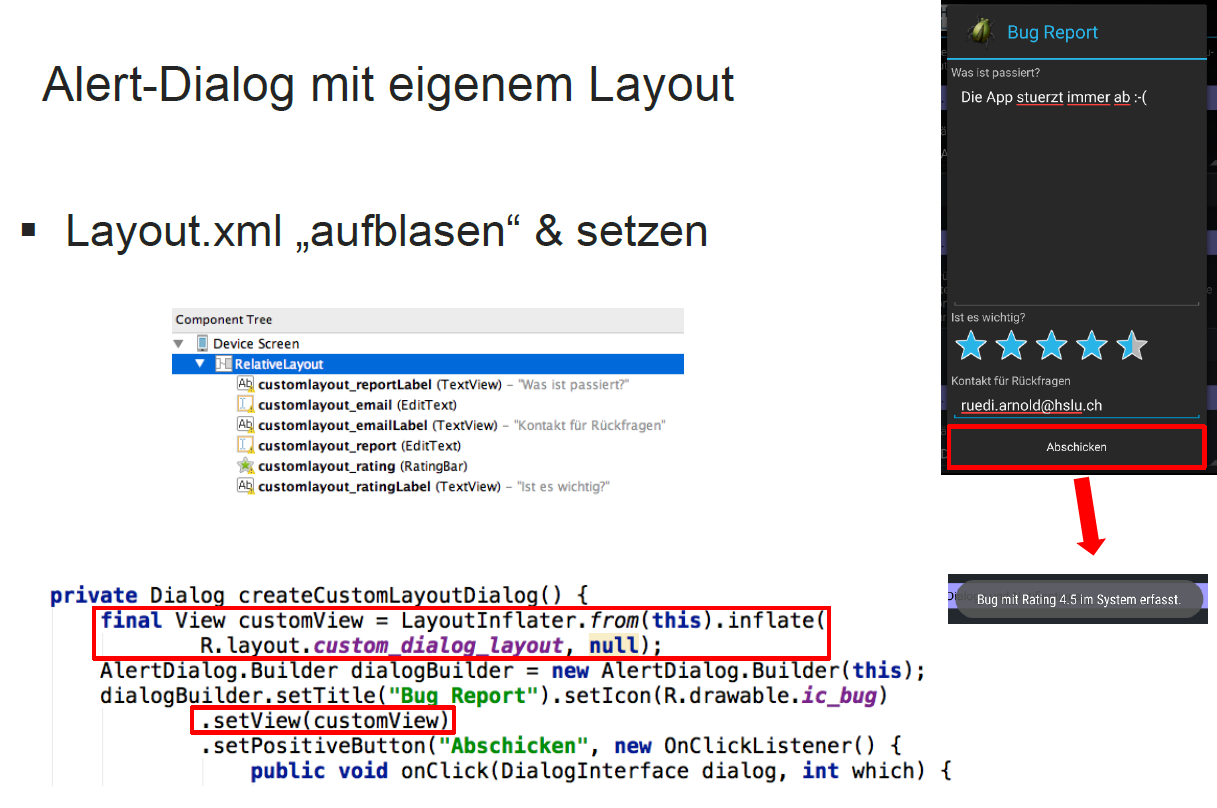
\includegraphics[width=\textwidth]{img/alertdialog_custom.png}
	\caption{Beispiel mit eigenem Layout}
\end{figure}

\newpage
\noindent
Ein (offener) Dialog gehört zum Zustand einer Activity, ist ein Dialog noch geöffnet bei einem Konfigurationswechsel, dann wird dieser nicht gespeichert und auch nicht wiederhergestellt! Deshalb sollten Dialoge als \texttt{DialogFragment} implementiert werden. Der Zustand des Dialogs wird dann vom \texttt{FragmentManager} korrekt mit Lifecycle und Activity synchronisiert (save/restore)\\
Für den Moment: Ein \textbf{Fragment} ist ein wiederverwendbarer "UI Schnippsel" mit eigenem Zustand und Lifecycle.

\subsubsection{Notifications (Status-Bar)}

\begin{itemize}
	\item Persistente Nachricht
	\begin{itemize}
		\item Kurze Ticker-Nachricht in der Status-Bar
		\item Danach persistente Anzeige im Notification Window
		\item Bei Auswahl erfolgt Aufruf einer definierten Activity
	\end{itemize}
	\item Vorteile:\\
	Nachricht bleibt erhalten bis vom Nutzer quittiert\\
	Beliebig komplexe Behandlung, da Start einer Activity
	\item Nachteil:\\
	Etwas komplexere Mechanik wegen \texttt{PendingIntent}
\end{itemize}

\begin{figure}[htb!]
	\centering
	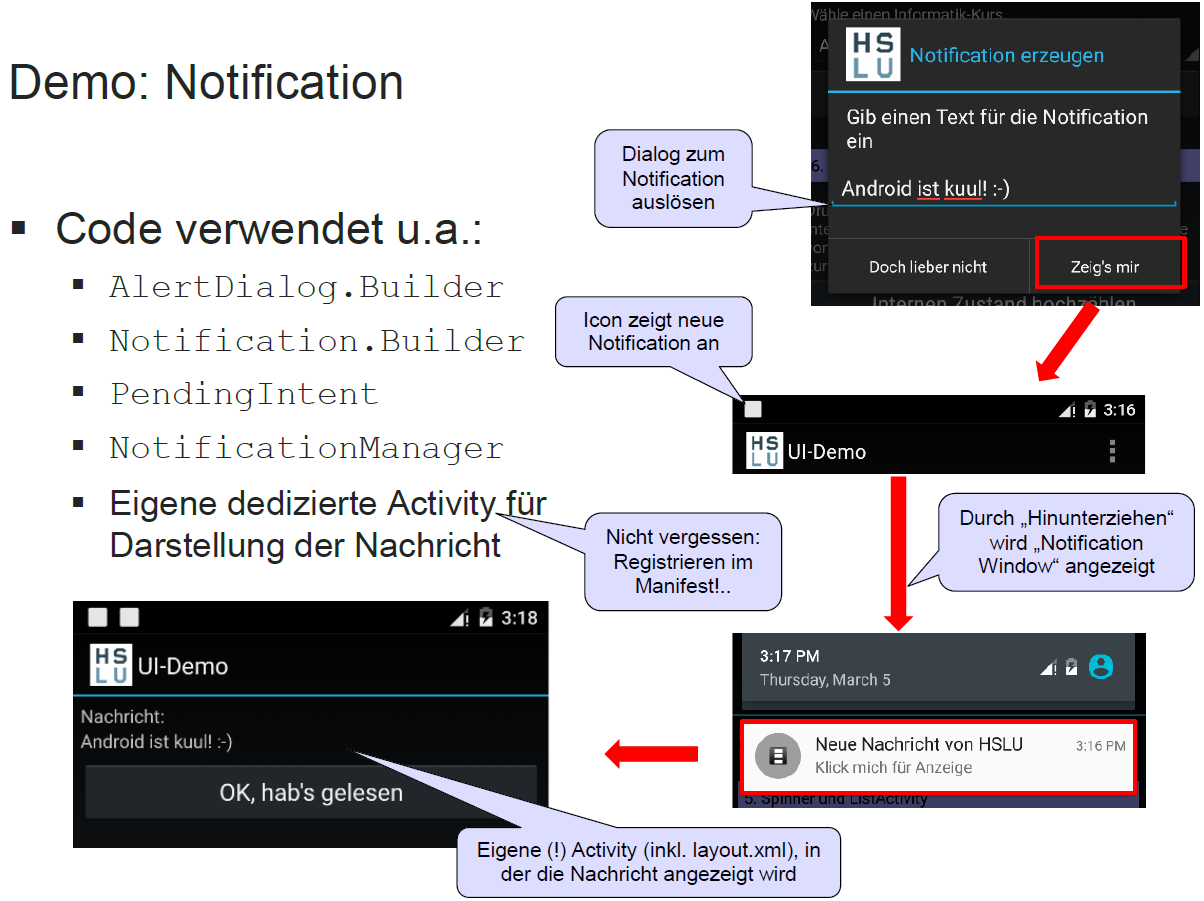
\includegraphics[width=\textwidth]{img/notification_demo.png}
	\caption{Übungs-Demo aus der Vorlesung SW02 - Notification}
\end{figure}

\newpage
\section{Android 3 - Persistenz \& Content Providers}

Persistenz: Daten über Laufzeit der App erhalten.
Für lokale Persistenz gibt es drei Möglichkeiten:
\begin{itemize}
	\item \textbf{Shared Preferences}\\
	Key/Value-Paare, Verwendung für kleine Datenmengen
	\item \textbf{Dateisystem}\\
	intern oder extern, in App-Sandbox (privat) oder auf SD-Karte (öffentlich), Verwendung für binäre/grosse Dateien, Export
	\item \textbf{Datenbank (Room)}\\
	SQLite + Object Relational Mapper (ORM), Verwendung für strukturierte Daten + Abfragen/Suche
\end{itemize}

\subsection{(Shared) Preferences}
\begin{itemize}
	\item Jede Activity hat ein SharedPreferences-Profil, persistente Einstellungen für Activity oder Applikation
	\item Key-Value-Store (persistente Map)
	\item Preferences für \textbf{Activity}: \\
	\texttt{Activity.getPreferences(mode)}\\
	Anwendungsfall: Activity-State persistent speichern
	\item Preferences für \textbf{Applikation}: \\
	\texttt{PreferenceManager.getDefaultSharedPreferences(ctx)}\\
	\texttt{Context.getSharedPreferences(name, mode)}
	\item Mögliche Datentypen für Preferences-Werte:\\
	\textit{String, int, float, long, boolean, Set<String>} (mit seperaten Werten)
\end{itemize}
\paragraph{Lesen und Schreiben auf Preferences}
\begin{itemize}
	\item Mehrere Dateien pro Applikation möglich, Zugriff mit\\
		\texttt{Activity.getSharedPreferences(name, mode)} (unterschiedliche Dateinamen)\\
		oder auch über \texttt{getDefaultSharedPreferences(mode)}, die Applikation findet danach anhand der Preference-Benennungen die Einträge auch selber
	\item Lesen mit Methoden \texttt{SharedPreferences.get\textbf{X}()}\\
		\textbf{X} steht für den Typ, also String, Int, Boolean, ...
	\item Schreiben immer mit dem Editor:
		\begin{enumerate}
			\item \texttt{SharedPreferences.Editor editor = preferences.edit()}
			\item \texttt{editor.put\textbf{X}(...)}
			\item \texttt{editor.apply()} Persistierung der Änderungen
				\begin{itemize}
					\item asynchrone Persistierung, blockiert die Methode nicht
					\item für synchrone Persistierung: \texttt{editor.commit()}
				\end{itemize}
		\end{enumerate}
\end{itemize}
\vspace{1em}
Beispiel, um die Anzahl Aufrufe einer App über die Lebenszeit der App hinaus zu persistieren:

\begin{lstlisting}
final SharedPreferences preferences = getPreferences(MODE_PRIVATE);
final int newResumeCount = preferences.getInt(COUNTER_KEY, 0) + 1;
final SharedPreferences.Editor editor = preferences.edit();
editor.putInt(COUNTER_KEY, newResumeCount);
editor.apply();
\end{lstlisting}

\subsubsection{Darstellung User-Preferences}

	\begin{itemize}
		\item Automatische Darstellung mit \texttt{PreferenceFragment}, eigener Editor für jeden Wertetyp
		\item \texttt{PreferenceFragment} schreibt/liest grundsätzlich in die DefaultSharedPreferences, kann aber auch für andere Preference-Stores konfiguriert werden
	\end{itemize}

\newpage
\noindent
User-Präferenzen können in XML deklariert werden unter \texttt{res/xml} z.Bsp. als \texttt{preferences.xml}, wobei untersch. Präferenzen bspw. als \texttt{CheckBoxPreference, ListPreference} usw. erfasst werden. Daten können wie in diesem Beispiel aus den Array-Ressourcen bezogen werden:

\begin{figure}[htb!]
	\centering
	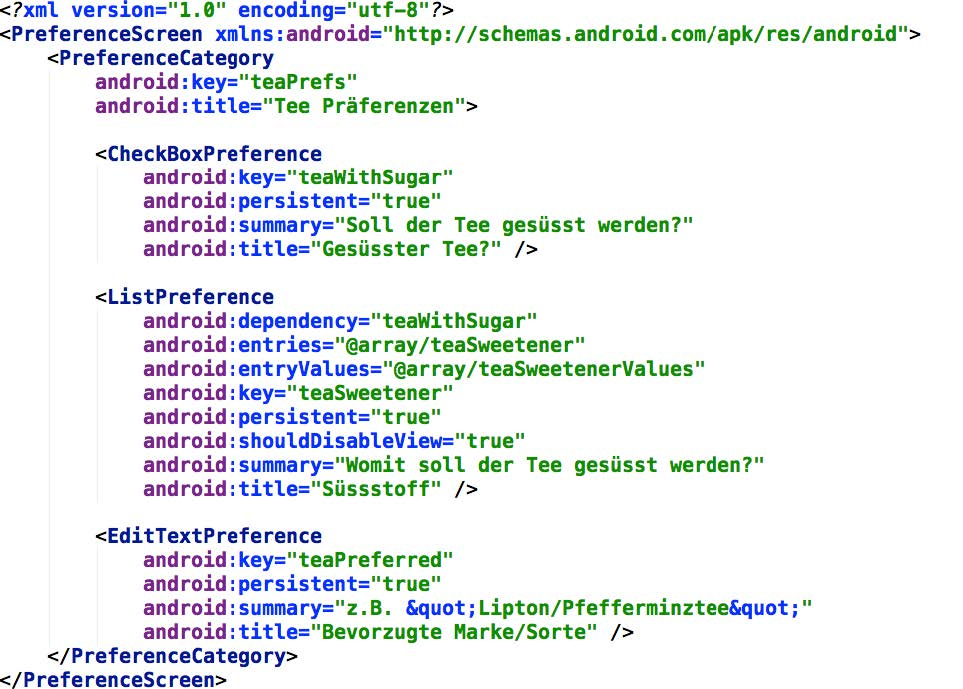
\includegraphics[width=.7\textwidth]{img/prefs_xml.jpg}
	\caption{Beispiel eines Präferenzen-XML}
\end{figure}

\begin{itemize}
	\item Ohne \texttt{android:summary} würde die gewählte Preference angezeigt werden
	\item \texttt{android:dependency} deklariert eine Abhängigkeit zu einer anderen Preference, ist diese nicht gegeben kann die andere Preference nicht ausgewählt werden
	\item \textbf{Entries}: "Anzeigestring", übersetzbar\\
	\textbf{EntryValues}: "Werte", nicht übersetzt, technischer Schlüssel
\end{itemize}
\begin{lstlisting}
// Zur "Uebersetzung" von Values zu Entries (Beispiel)
public String getValueFromKey(String key) {
	String[] keys = getResources().getStringArray(R.array.teaSweetenerValues);
	String[] values = getResources().getStringArray(R.array.teaSweetener);
	int i = 0;
	while(i < keys.length) {
		if(keys[i].equals(key)) {
			return values[i];
			}
		i++;
	}
	return "";
}
\end{lstlisting}

\newpage

\subsubsection{PreferenceFragment}

Ein \texttt{PreferenceFragment} kann in einer eigenen Activity (hier \texttt{TeaPreferenceActivity}) erstellt werden:

\begin{lstlisting}
public class TeaPreferenceActivity extends Activity {

	@Override
	protected void onCreate(Bundle savedInstanceState) {
		super.onCreate(savedInstanceState);
		getFragmentManager().beginTransaction().replace(android.R.id.content,
			new TeaPreferenceInitializer()).commit();
	}
	
	// PreferenceFragment als statische innere Klasse
	public static final class TeaPreferenceInitializer extends PreferenceFragment {
		@Override
		public void onCreate(final Bundle savedInstanceState) {
			super.onCreate(savedInstanceState);
			addPreferencesFromResource(R.xml.preferences);
			// Referenz auf preferences.xml
	}
}
\end{lstlisting}

\subsubsection{Default-Präferenzen}

Präferenzen können programmatisch auch wieder auf "Standard"-Werte oder auf festgelegte Werte gesetzt werden, für das Tee-Beispiel kann dies bspw. folgendermassen vorgenommen werden:

\begin{lstlisting}
SharedPreferences teaPrefs = PreferenceManager.getDefaultSharedPreferences(this);
SharedPreferences.Editor editor = teaPrefs.edit();
editor.putString("teaPreferred", "Lipton/Pfefferminztee");
editor.putString("teaSweetener", "natural");
editor.putBoolean("teaWithSugar", true);
editor.apply();
\end{lstlisting}

\newpage
	
\subsection{Dateisystem}

\begin{itemize}
	\item \textbf{Einsatzbereiche}
		\begin{itemize}
			\item Speichern/Laden von binären Dateien (Bilder, Musik, Video, Java-Objects, etc.)
			\item Caching (Heruntergeladene Dateien)
			\item Grosse Text-Dateien(Plain Text, Strukturierte Daten wie XML, JSON,))
		\end{itemize}
	\item Teilen / Freigeben von erstelltem Inhalt (Externer Speicher wie SD-Karte)
\end{itemize}

\begin{itemize}
	\item Dateien sind entweder
	\begin{itemize}
		\item PRIVATE $\rightarrow$ ins Applikationsverzeichnis\\
		\textit{(Zugriff für andere Apps nur über Content Provider möglich)}
		\begin{itemize}
			\item \texttt{Context.getFilesDir()}
		\end{itemize}
		\item PUBLIC $\rightarrow$ auf die SD-Karte 
		\begin{itemize}
			\item \texttt{Environment.getExternalStorageDirectory()}\\
			\texttt{Environment.getExternalStorageState();}
		\end{itemize}
	\end{itemize}
	\item Für Zugriff auf SD-Karte muss die Permission im Manifest eingetragen werden! (siehe nachfolgend)
\end{itemize}
	
\subsubsection{Exkurs: Permission-Model}

	\begin{itemize}
		\item Vor gewissen Operationen müssen Apps die Berechtigung des Nutzers erhalten (Kontaktzugriff, Internet, SD-Karte, Kamera, SMS, etc.)
		\item Klasse: \texttt{android.Manifest.permission}
		\item Seit API 23 werden keine dangerous Permissions mehr gewährt, der Nutzer muss diese selber freigeben (Applikation fragt beim Nutzer nach), Permissions werden einzeln gewährt/abgelehnt.\\
		\textbf{Konsequenz}: Apps müssen mit eingeschränkten Permissions umgehen können
		\item Arten von Permissions
		\begin{itemize}
			\item \textit{normal}
				\begin{itemize}
					\item Wird bei der Installation automatisch erlaubt
				\end{itemize}
			\item \textit{dangerous}
				\begin{itemize}
					\item Muss von User erlaubt werden (kann wieder entzogen werden)
				\end{itemize}
			\item \textit{signature}
				\begin{itemize}
					\item Wird automatisch erlaubt, wenn die App, welche die Permission definiert, vom gleichen Hersteller ist wie die App, welche die Permission beanträgt (sonst ist sie "dangerous")
				\end{itemize}
			\item \textit{signatureOrSystem}
				\begin{itemize}
					\item Wird automatisch erlaubt für Apps, welche im System-Image sind, sonst wie "signature"
				\end{itemize}
		\end{itemize}
		\item Permissions können gruppiert werden, User gibt Freigabe für alle Permissions in einer Gruppe (keine einzelnen Permissions), falls benötigt
	\end{itemize}
	
	\begin{figure}[htb!]
		\centering
		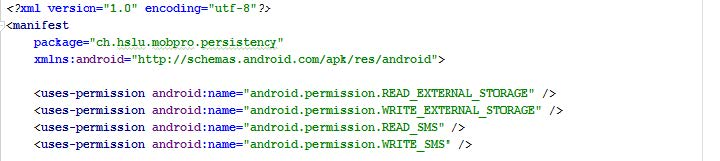
\includegraphics[width=.7\textwidth]{img/manifest_permissions.jpg}
		\caption{Erfassung von Permissions im Manifest}
	\end{figure}

\newpage

	\subsubsection{Exkurs ff: Runtime Permissions}
	
	\begin{figure}[htb!]
		\centering
		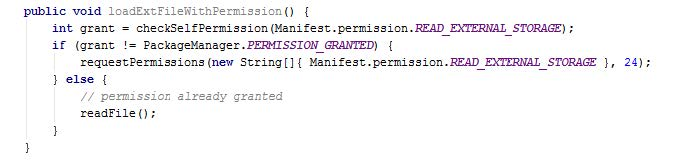
\includegraphics[width=.9\textwidth]{img/runtimeperm1.jpg}
		\caption{RuntimeCheck der Permissions}
	\end{figure}
	
	\begin{figure}[htb!]
		\centering
		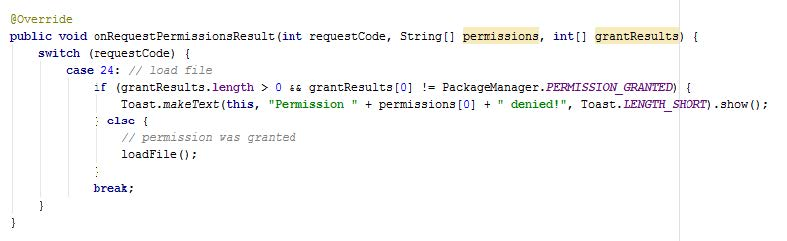
\includegraphics[width=.9\textwidth]{img/runtimeperm2.jpg}
		\caption{Callback aus Permission-Abfrage}
	\end{figure}
	
	\subsubsection{Exkurs ff: Persistenz mit Datei}
	
	Repetition zu Streams, Reader \& Co.
	
	\begin{itemize}
		\item Stream: Byte-Datenstrom \texttt{[28,11,200,255,2,15,33]}
			\begin{itemize}
				\item Auf \texttt{File} öffnen:\\
				\texttt{FileOutputStream, FileInputStream}
			\end{itemize}
		\item Stream kann in Zeichenstrom \texttt{['h','a','l','l','o']} umgewandelt werden
			\begin{itemize}
				\item \texttt{FileReader, FileWriter} + "Buffered"-Versionen
			\end{itemize}
		\item Immer schliessen!\\
		\texttt{stream.close() / reader.close()}
		\item Nicht vergessen: \texttt{try-catch-finally} implementieren
		\item \texttt{java.nio.file.Path}: ist ab API 26 in Android verfügbar!
	\end{itemize}

	\begin{figure}[htb!]
		\centering
		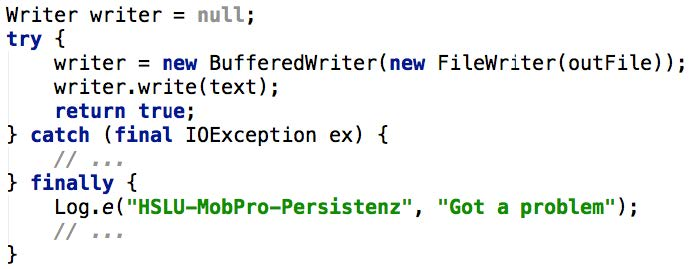
\includegraphics[width=.7\textwidth]{img/persist_text.jpg}
		\caption{Beispielcode zur Persistierung in einem Textfile}
	\end{figure}

\newpage	
	
\subsection{Datenbank (Room)}

Android-DB \textbf{SQLite} ist bei Android fix integriert. Ein DB-Adapter ist die Verbindung zwischen Business-Objekten und einer Datenbank.

\begin{figure}[htb!]
	\centering
	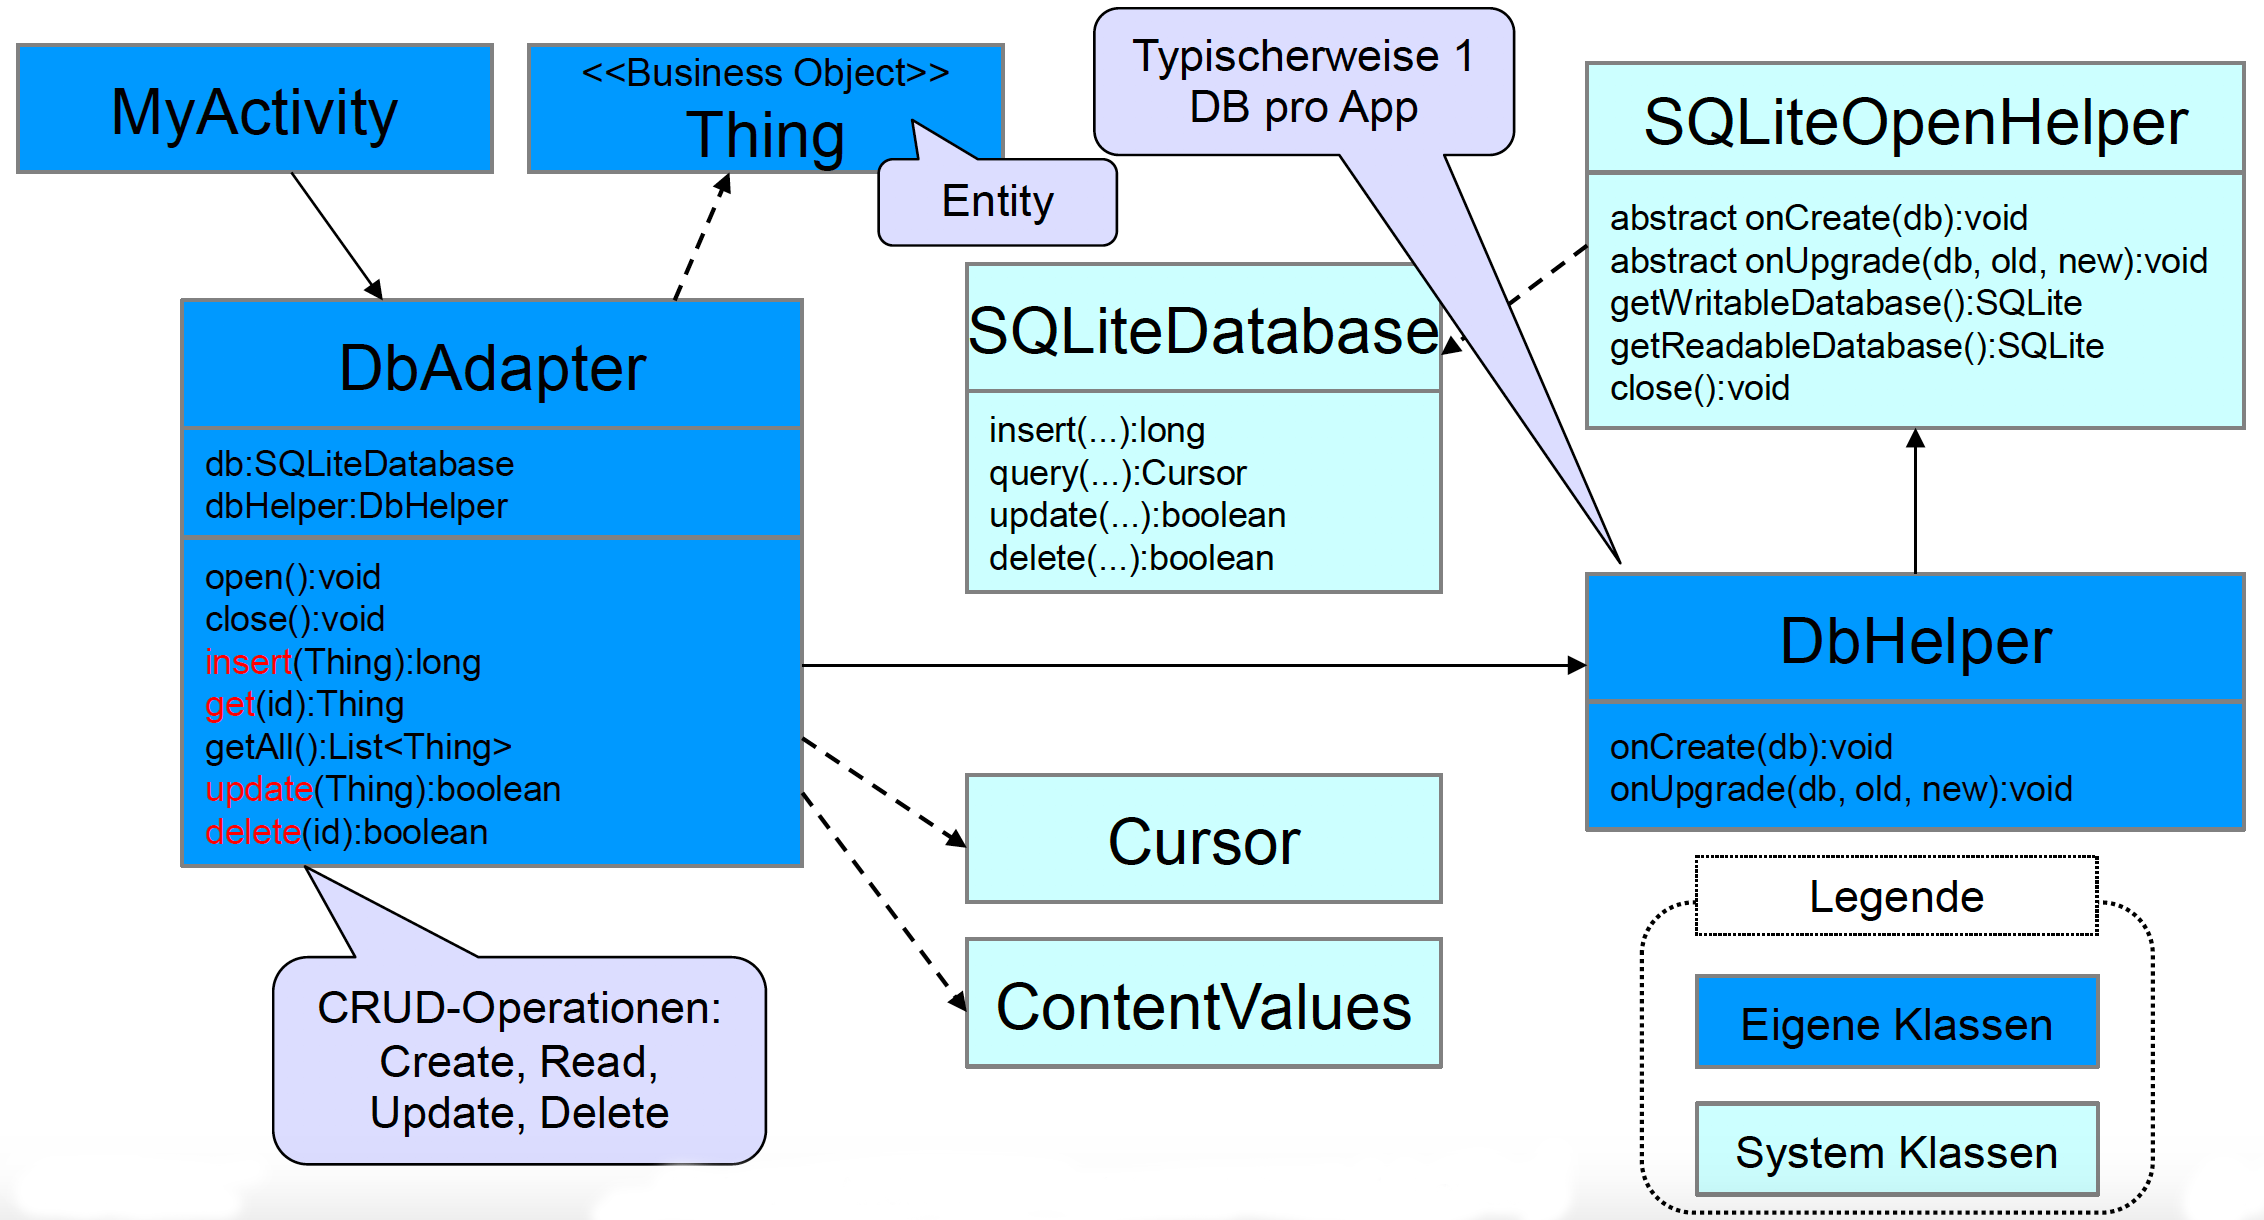
\includegraphics[width=.85\textwidth]{img/sqlite_framework.png}
	\caption{SQLite Framework}
\end{figure}

\begin{itemize}
	\item Room ist ein Object Relational Mapper (ORM) für Android
		\begin{itemize}
			\item Klassen werden auf relationale DB-Tabellen gemappt
			\item Zugriff auf Datenbank wird abstrahiert\\
			$\rightarrow$ Typischerweise werden SQL-Statements durch Methodenaufrufe gekapselt
		\end{itemize}
	\item Spezialfälle des Room ORM
		\begin{itemize}
			\item \textit{Datenzugriff über DAO}: Queries werde als SQL-Statements in Annotationen definiert
			\item Beziehungen zwischen Entitäten müssen manuell abgebildet werden (Performance!)
			\item \textit{Nested Objects}: mehrere POJOs in einer Tabelle
			\item Einschränkungen für Datenzugriffe, standardmässig nicht möglich im UI Thread
		\end{itemize}
	\item Die drei Komponenten von Room
		\begin{description}
			\item[Database] Abstraktion der Datenverbindung
			\item[Entity] Repräsentation einer Tabelle in der relationalen DB
			\item[DAO] (Data Access Object) Enthält Methoden für Datenzugriff
		\end{description}
\end{itemize}

\begin{figure}[htb!]
	\centering
	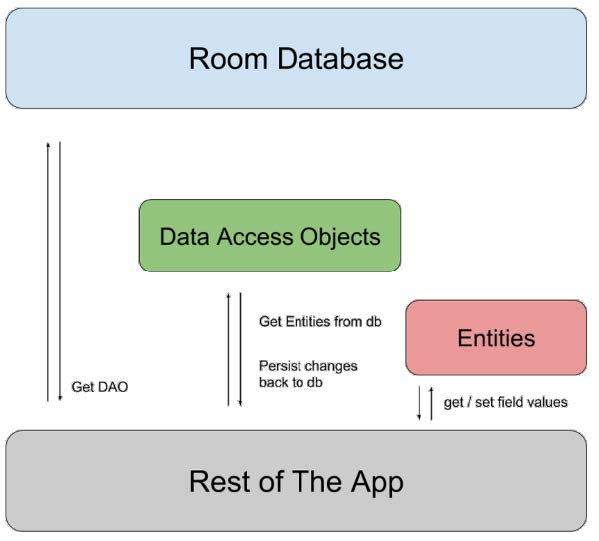
\includegraphics[width=.5\textwidth]{img/room_components.jpg}
	\caption{Komponenten von Room}
\end{figure}

\newpage

\subsubsection{Room - Code-Beispiele}

\begin{lstlisting}
@Entity // POJO mit Annotationen
public class User {
	@PrimaryKey
	public int uid;
	
	@ColumnInfo(name = "first_name")
	public String firstName;
	
	@ColumnInfo(name = "last_name")
	public String lastName;
}
\end{lstlisting}

\begin{lstlisting}
@Dao // Datenzugriff ueber Annotationen (teilweise mit SQL-Queries)
public interface UserDao {
	@Query("SELECT * FROM user") 
	List<User> getAll(); 
	
	@Query("SELECT * FROM user WHERE uid IN (:userIds)") 
	List<User> loadAllByIds(int[] userIds); 
	
	@Insert 
	void insertAll(User... users); 
	
	@Delete 
	void delete(User user);
}
\end{lstlisting}

\begin{lstlisting}
// Database: Subklasse von RoomDatabase, konfiguriert mit Database Annotation
@Database(entities = {User.class}, version = 1)
public abstract class AppDatabase extends RoomDatabase {
	public abstract UserDao userDao();
}

// Zum Erzeugen einer Instanz der DB:
AppDatabase db = Room.databaseBuilder(
			getApplicationContext(),
			AppDatabase.class,
			"database-name"
).build();
\end{lstlisting}

\newpage

\subsubsection{Room - Daten mit Entitäten definieren}

\begin{itemize}
	\item Ein POJO mit \texttt{@Entity} Annotation
	\item Primärschlüssel (wird in jeder Entität benötigt)
		\begin{itemize}
			\item \texttt{@PrimaryKey} für ein einzelnes Feld, optional mit \texttt{autoGenerate} Property
			\item Für zusammengesetzte Primärschlüssel:\\
			\texttt{primaryKeys} Property in \texttt{@Entity} Annotation
		\end{itemize}
	\item Falls bestimmte Felder nicht gespeichert werden sollen
		\begin{itemize}
			\item \texttt{@Ignore} Annotation für ein einzelnes Feld
			\item mit \texttt{ignoredColumns} Property in \texttt{@Entity} Annotation für mehrere Felder \\
			(v.a. von Superklassen)
		\end{itemize}
\end{itemize}

\begin{lstlisting}
// Code-Beispiel
// ACHTUNG: dieses Beispiel definiert mehrere Primary Keys und vermischt Ansaetze zum Ignorieren von Feldern zwecks Syntax-Demonstration!

@Entity(primaryKeys = {"firstName", "lastName"},
			ignoredColumns = "password, otherField")
public class User extends Party {
	@PrimaryKey(autoGenerate = true)
	public int id;
	
	public String firstName;
	public String lastName;
	
	@Ignore
	Bitmap picture;
}
\end{lstlisting}

\subsubsection{Room - Beziehungen modellieren}

\textbf{Beachte:} Room erlaubt aus Performanzgründen keine Objektreferenzierungen!

\begin{lstlisting}
@Entity(foreignKeys = @ForeignKey(entity = User.class,
															parentColumns = "id",
															childColumns = "user_id"))
public class Book {
	@PrimaryKey
	public int bookId;
	
	public String title;
	
	@ColumnInfo(name = "user_id"
	public int userId; // Feld-Typ: nur ID, nicht User
}
\end{lstlisting}

\newpage

\subsection{Mit DAOs auf Daten zugreifen}

\begin{itemize}
	\item DAOs enthalten Methoden für den abstrahierenden Datenbankzugriff
	\item Trägt zur \textit{Separation of Concerns} bei und erhöht die Testbarkeit\\
	$\rightarrow$ DAOs können gemockt werden!
	\item DAOs als Interfaces oder abstrakte Klassen definieren\\
	$\rightarrow$ Room erzeugt passende Implementationen bei der Kompilierung\\
	\textit{(Typischerweise eine DAO-Klasse pro Entity, mit allen möglichen Operationen)}
	\item Zwei Möglichkeiten:\\
	Convenienve Queries \textbf{oder} \texttt{@Query} Annotation mit SQL-Statements
\end{itemize}

\subsubsection{Convenience Queries}

\begin{itemize}
	\item Werden über Annotations für die jeweiligen Methoden definiert:\\
	\texttt{@Insert, @Update, @Delete}
	\item Alle Parameter müssen Klassen mit einer \texttt{@Entity} Annotation \\
	(oder Collections/Arrays) davon sein
	\item Rückgabewerte:
		\begin{itemize}
			\item \textbf{Insert}: \texttt{long} bzw. \texttt{long[]} bzw. \texttt{List<Long>} \textit{(liefert Row-IDs zurück)}
			\item \textbf{Update / Delete}: \texttt{int} \textit{(Anzahl modifizierte Tabelleneinträge)}
		\end{itemize}
	\begin{lstlisting}
@Insert
public long[] insertUsersAndFriends(User user, List<User> friends);
		// ID Rueckgabe, sonst void
															// Parameter fuer Operation (Entities)
	\end{lstlisting}
\end{itemize}

\begin{lstlisting}
// Weitere Convenience Queries Beispiele

@Dao
public interface MyDao {

	@Insert (onConflict = OnConflictStrategy.REPLACE)
	public void insertUsers(User... users);
	@Insert
	public void insertBothUsers(User user1, User user2);
	@Insert
	public long[] insertUsersAndFriends(User user, List<User> friends);
	
	@Update
	public void updateUsers(User... users);
	
	@Delete
	public void deleteUsers(User... users);
}	
\end{lstlisting}

\newpage

\subsubsection{Custom Queries mit @Query}

\begin{itemize}
	\item DIe \texttt{@Query} Annotation kann für Schreib- und Lesevorgänge genutzt werden
	\item Jede \texttt{@Query} wird zur Kompilierzeit überprüft\\
	$\rightarrow$ Kompilierfehler bei ungültigen Queries, keine Laufzeitfehler!
	\item Für eine \texttt{@Query} kann eine beliebige Anzahl (0..n) Parameter verwendet werden
	\item Wenn nicht ganze Objekte benötigt werden, können Ressourcen gespart werden durch die Verwendung von POJOs mit \texttt{@ColumnInfo} Annotationen
\end{itemize}

\begin{lstlisting}
// Custom Queries Codebeispiele

@Dao 
public interface MyDao { 
	@Query("SELECT * FROM user") 
	public User[] loadAllUsers();

	@Query("SELECT * FROM user WHERE age > :minAge") 
	public User[] loadAllUsersOlderThan(int minAge);

	@Query("SELECT first_name, last_name FROM user WHERE region IN (:regions)") 
	public List<NameTuple> loadUsersFromRegions(List<String> regions); 
}

public class NameTuple { 
	@ColumnInfo(name = "first_name") 
	public String firstName;

	@ColumnInfo(name = "last_name") 
	public String lastName; 
}
\end{lstlisting}

\newpage

\subsection{DB-Einträge in einer Liste anzeigen}

\begin{itemize}
	\item Verschiedene Ansätze, je nach Umfang/Komplexität der Datensätze:\\
	ListView, RecyclerView, Kombination mit ViewModel und LiveData
	\item In jedem Fall werden spezifische Adapter benötigt, um die Daten auf Views zu mappen
\end{itemize}

\begin{figure}[htb!]
	\centering
	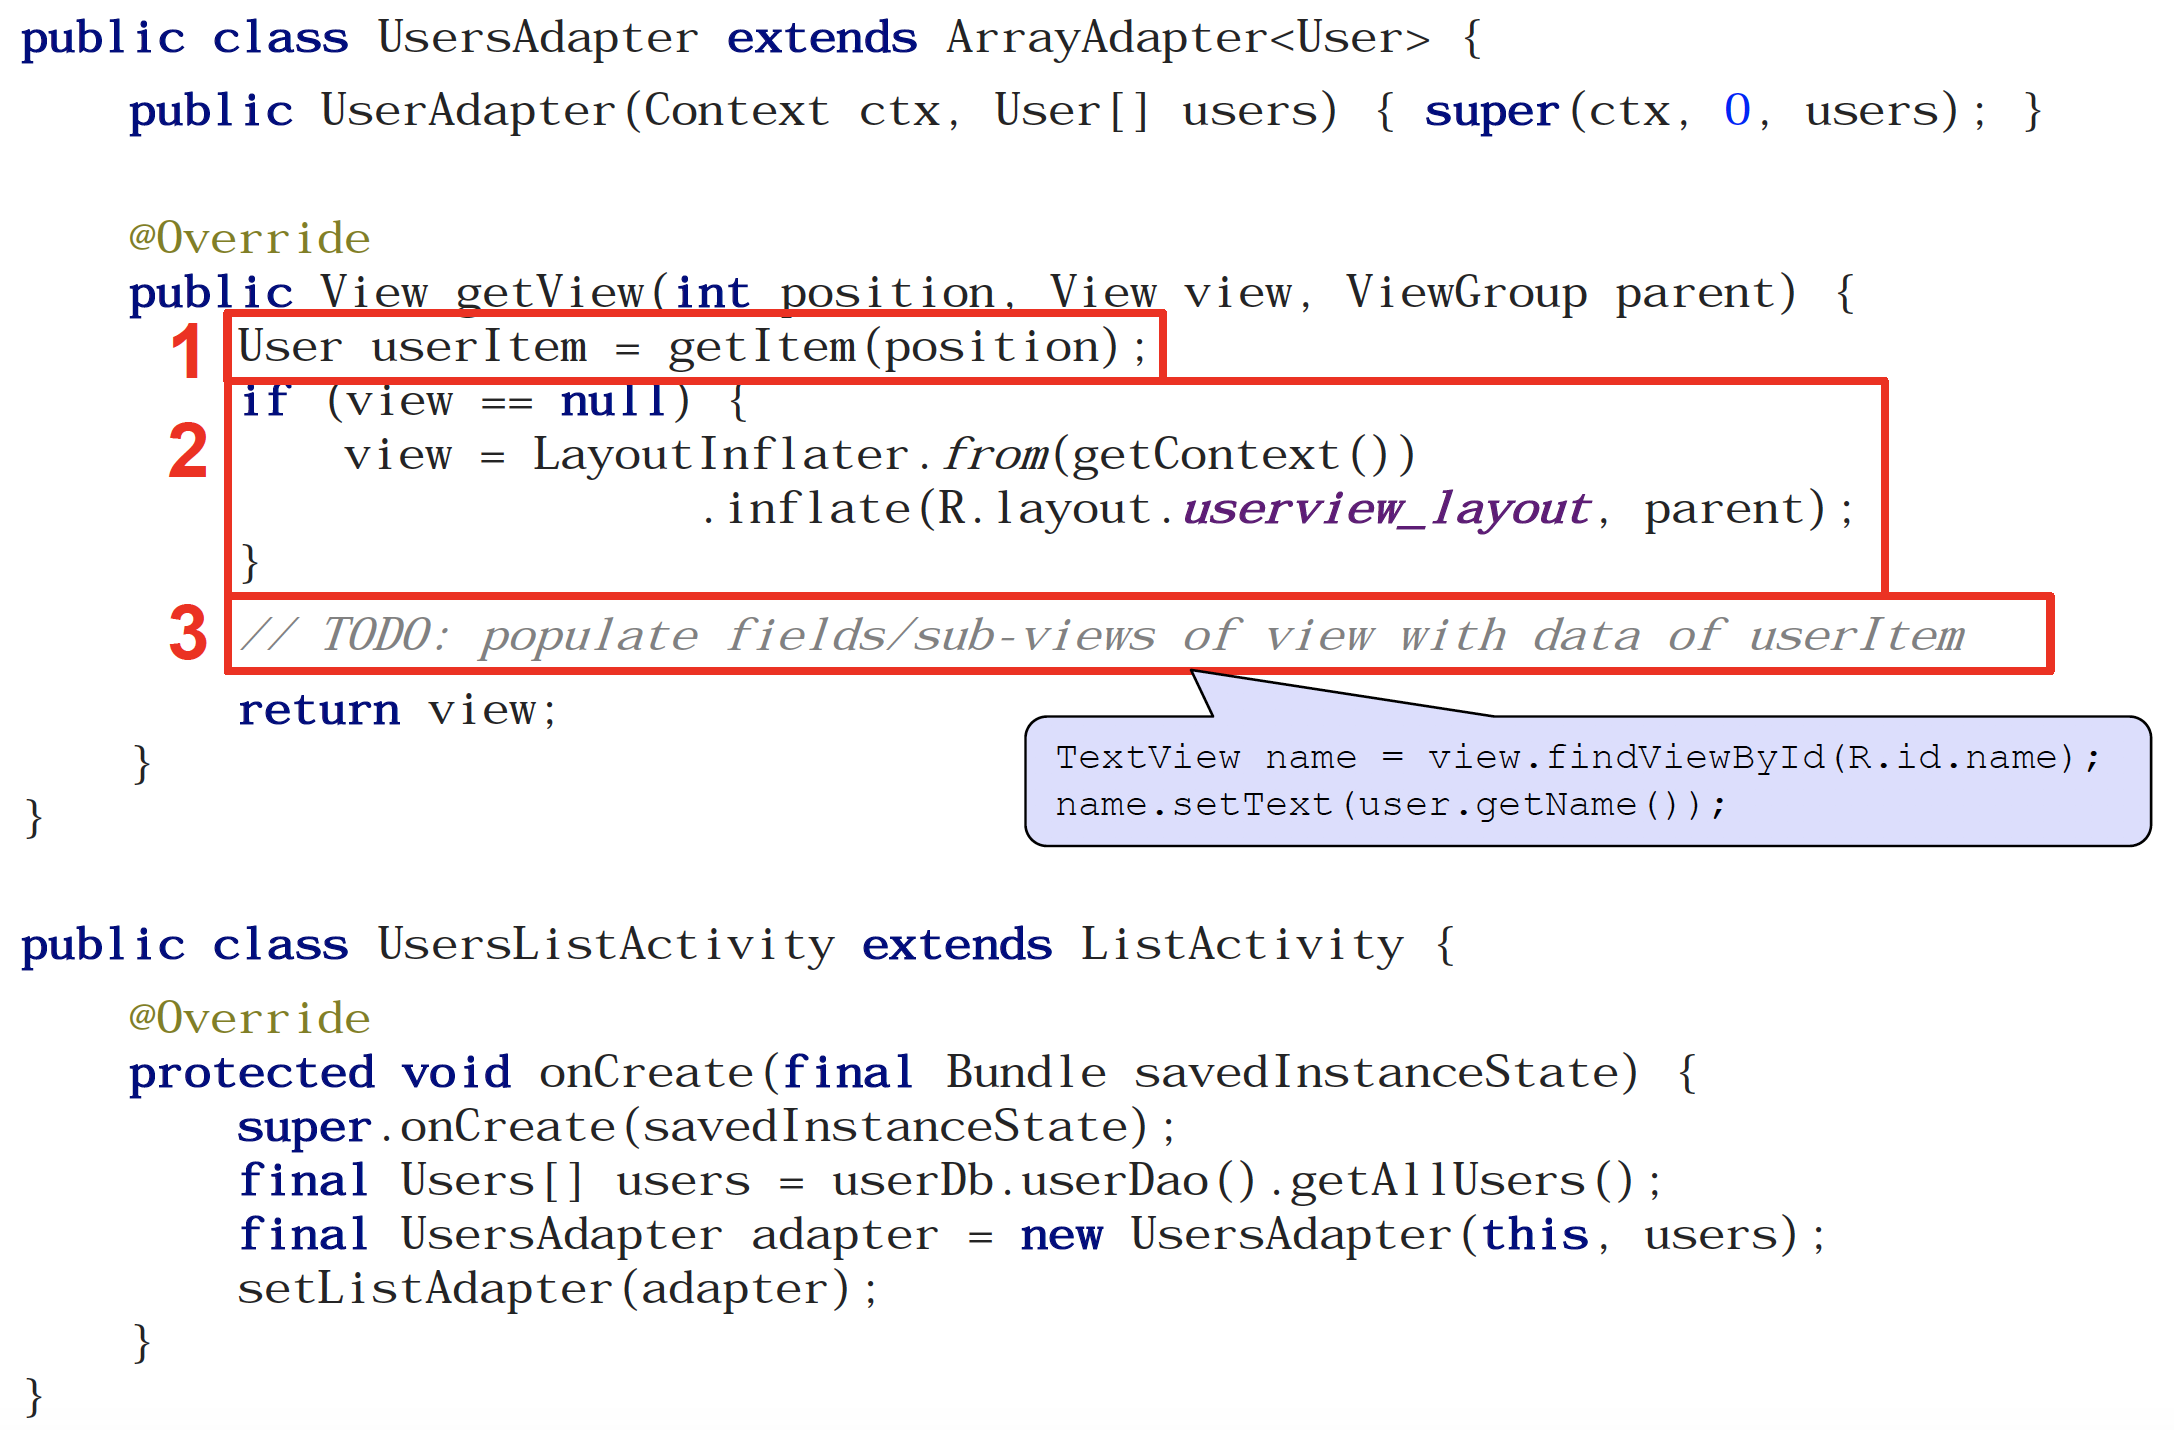
\includegraphics[width=\textwidth]{img/dbentries_list.png}
	\caption{Codebeispiel für das Darstellen von DB-Einträgen in einer Liste}
\end{figure}

\newpage

\subsection{Content Providers}

\begin{itemize}
	\item Content Provider stellen für andere Applikationen Daten bereit
	\item Die Daten stammen aus einer gekapselten DB \textbf{oder} aus dem privaten Dateisystem \textbf{oder} werden on-the-fly erzeugt
	\item Zugriff auf die Daten über URI (Uniform Ressource ID), Beispiel siehe in Abbildung \ref{fig:uri_content}
	\item Zwei Arten von URIs
		\begin{itemize}
			\item Pfad (Bezeichnete Datenmenge, vgl. Verzeichnit mit Daten)
			\item Item (Einzelnes Datenelement, vgl. einzelne Datei)
		\end{itemize}
\end{itemize}

\begin{figure}[htb!]
	\centering
	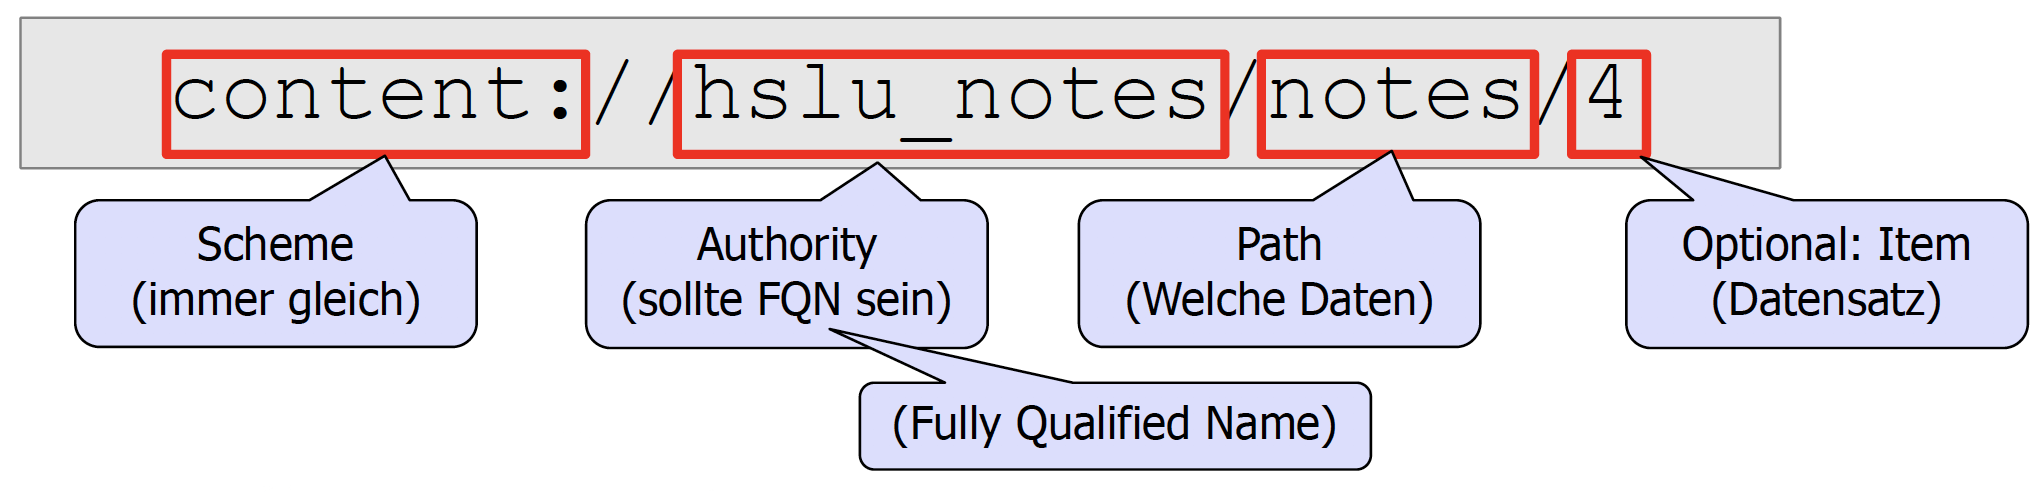
\includegraphics[width=.8\textwidth]{img/content_uri.png}
	\caption{Aufbau eines URI}
	\label{fig:uri_content}
\end{figure}
	
\subsubsection{Standard Content Providers}

\begin{itemize}
	\item Im Android-System gibt es bereits einige Content Providers, die genutzt werden können
		\begin{itemize}
			\item Kontakte: Namen, Telefon-Nummern, Emails, Adressen, etc.
			\item SMS/MMS: Erhaltene/Gesendete/Drafts SMS/MMS
			\item Media Store: Auf Gerät gespeicherte Audio-, Video-, Bilder-Daten
			\item Settings: Einstellungen für das Gerät
			\item Kalender: Kalender, Events, Erinnerungen, Teilnehmer, etc. 
		\end{itemize}
	\item Daten sind meist in mehreren Tabellen abgelegt
\end{itemize}	

\subsection{Exkurs : REST-ful Webservices}

\begin{itemize}
	\item Webservices auf der Basis von HTTP
	\item Grundidee (in purer Form)
		\begin{itemize}
			\item URL einer Ressourcensammlung \textit{(http://directory.com/contacts)}\\
			oder URL einzelner Ressource \textit{(http://directory.com/contacts/17)}
			\item HTTP-Methode = Operation auf Daten\\
			(GET, PUT, POST, DELETE)
			\item Antwort-Datenformat = XML, JSON, ...
		\end{itemize}
\end{itemize}

\begin{figure}[htb!]
	\centering
	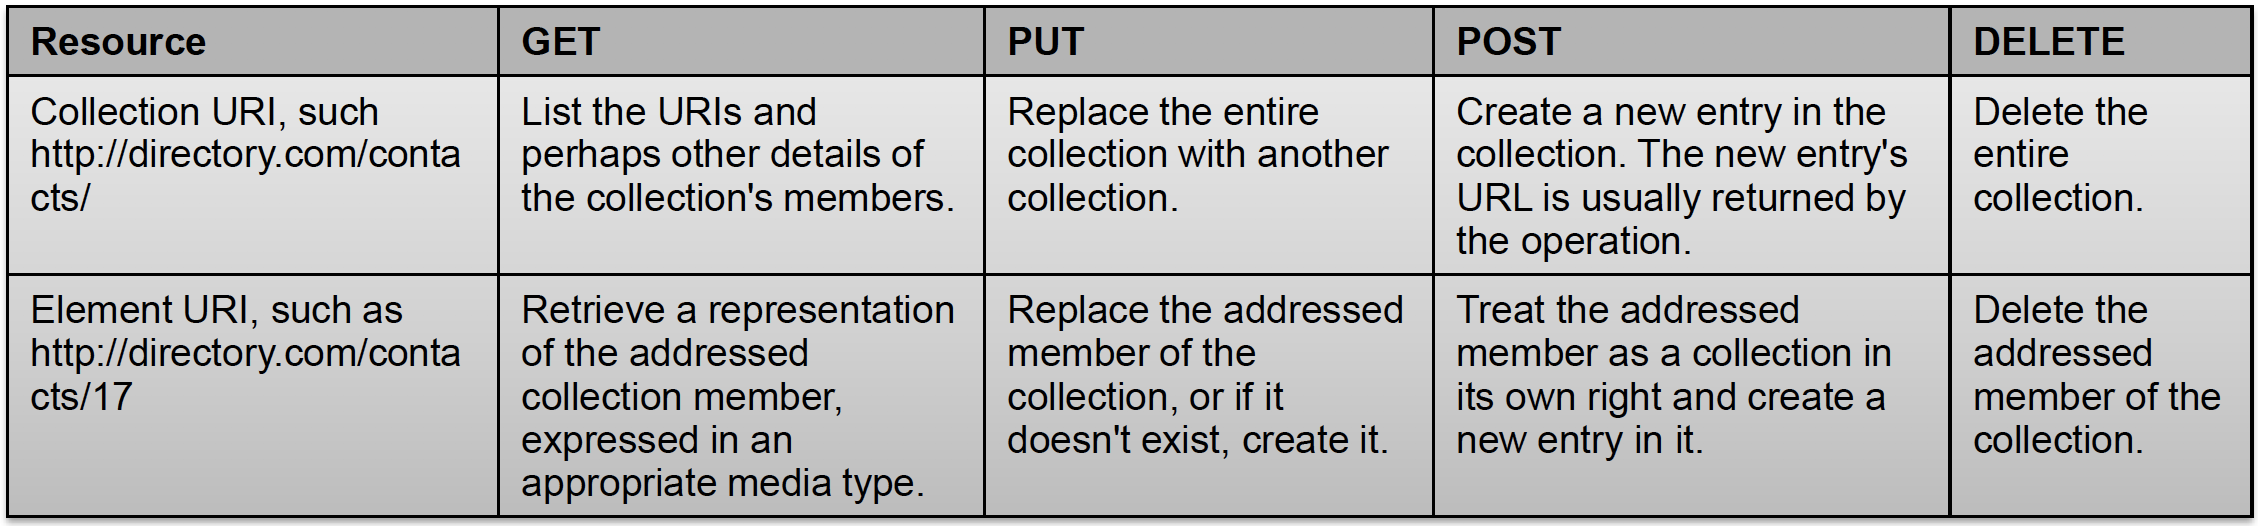
\includegraphics[width=\textwidth]{img/state_transfer.png}
	\caption{Beispiel - Representational State Transfer}
\end{figure}

\newpage

\subsection{Content Resolver \& Content Provider}

\begin{itemize}
	\item Zugriff auf einen Content Provider erfolgt über einen \textbf{Content Resolver}\\
	\texttt{Context.getContentResolver()}
		\begin{itemize}
			\item Bietet DB-Methoden und Zugriff auf Content via Streams
				\begin{itemize}
					\item CRUD: \texttt{insert() / query() / update() / delete()}
					\item \texttt{openInputStream(uri) / openOutputStream(uri)}
				\end{itemize}
			\item Ein Content Resolver ist ein Proxy, der...
				\begin{itemize}
					\item ...URI auflöst und zuständigen Content Provider sucht / findet
					\item ...Interprozess-Kommunikation behandelt (aufrufende App ist meist in einem anderen Package als der aufgerufene Content Provider)
				\end{itemize}
		\end{itemize}
	\item Unter Umständen müssen die Permissions noch gesetzt werden (im Manifest)
\end{itemize}
	
\subsubsection{Zugriff auf Daten über Content Resolver \& Query}	

\begin{lstlisting}
Cursor cursor = getContentResolver().query( 
		contentUri, 			// The content URI of the table 
		projection, 			// The columns to return for each row 
		selectionClause, 	// Selection criteria 
		selectionArgs, 		// Selection criteria 
		sortOrder); 			// The sort order for the returned row
\end{lstlisting}
	
\begin{figure}[htb!]
	\centering
	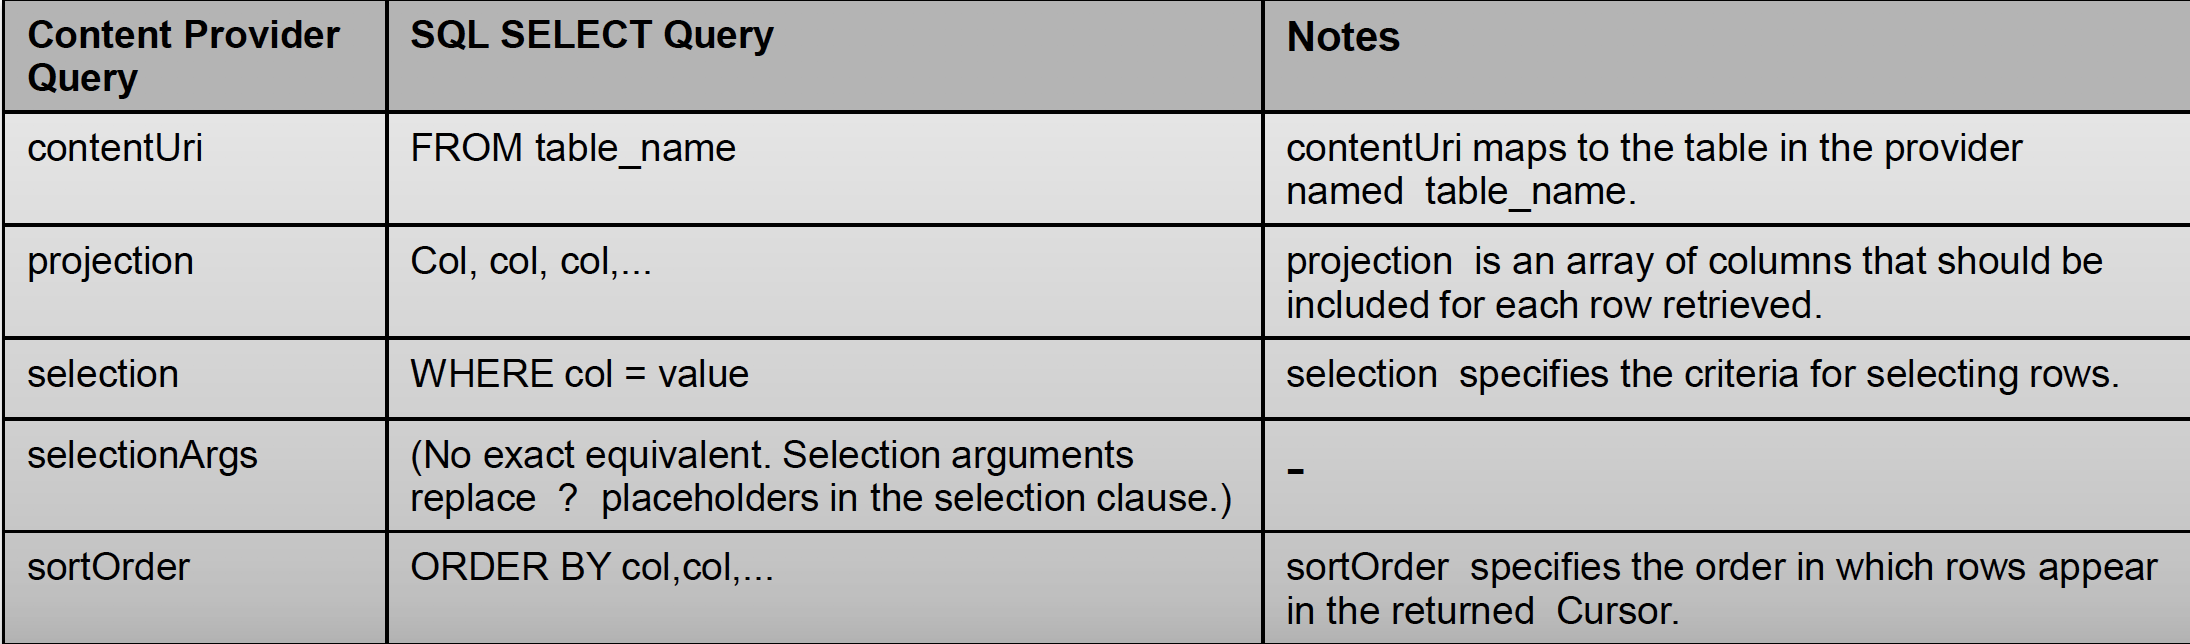
\includegraphics[width=\textwidth]{img/compare_query.png}
	\caption{Vergleich: ContentProvider Query und SQL Query Parameter}
\end{figure}

\begin{figure}[htb!]
	\centering
	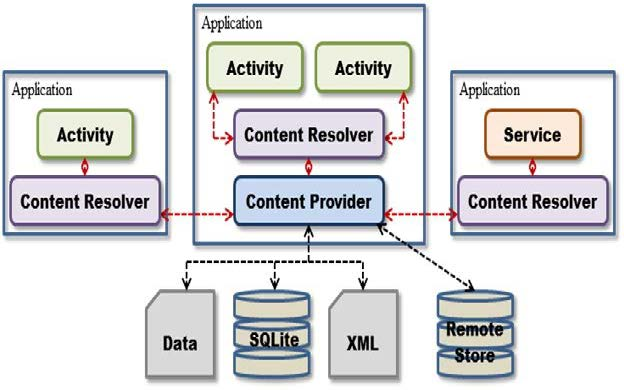
\includegraphics[width=.7\textwidth]{img/contentprovider.jpg}
	\caption{Content Provider - Anwendung (Data: Dateisystem, XML: Preferences)}
\end{figure}

\newpage

\begin{itemize}
	\item SMS des Systems sind über den Content Provider zugänglich\\
	\textit{(Benötigt Permission für SMS, diese testen und ggf. beantragen)}:
		\begin{itemize}
			\item \texttt{android.provider.Telephony.Sms}\\
			\textit{("Sub-Providers" für Sent, Inbox, Draft, etc.)}
			\item Im Package \texttt{android.provider.*} finden wir \\
			"Contract Klasse" \texttt{Telephone.Sms} mit \\
			Hilfsklassen \texttt{BaseColumns} und \texttt{Telephony.TextBasedSmsColumns}\\
			\textit{(Hier findet man Content-URI und Spalten-Namen für Projections)}
		\end{itemize}
\end{itemize}

\begin{figure}[htb!]
	\centering
	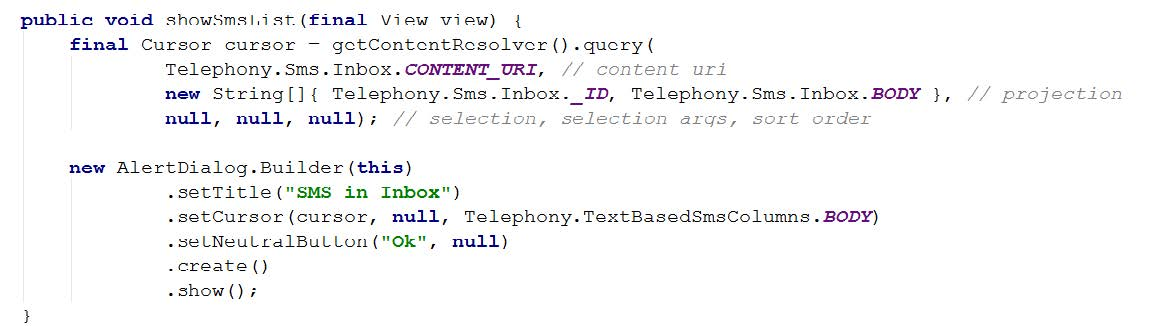
\includegraphics[width=\textwidth]{img/content_sms.jpg}
	\caption{Anwendungsbeispiel - Alle SMS mit Text anzeigen}
\end{figure}

Jeder Content Provider bietet eine eigene Standard-API, in der Android Dokumentation sind die Zugriffe auf Kontakte und Kalender gut dokumentiert (da dies eher komplizierte Modelle sind). Einstiegspunkt für die meisten Provider: \texttt{android.provider.*}

\subsection{Eigener Content Provider}

\begin{itemize}
	\item Um eigenen Content Provider zu schreiben, muss die eigene Klasse von der abstrakten Klasse\\ \texttt{android.content.ContentProvider} ableiten
	\item Wird bei App-Start hochgefahren und bleibt aktiv, in \texttt{onCreate()} kann eine Initialisierung vorgenommen werden (einzige Lifecycle-Methode)
	\item CRUD-Methoden: query, insert, update, delete (muss nicht alle implementieren)\\
	\textit{(Möglichkeit, einen read-only Content Provider anzulegen)}
\end{itemize}

\begin{figure}[htb!]
	\centering
	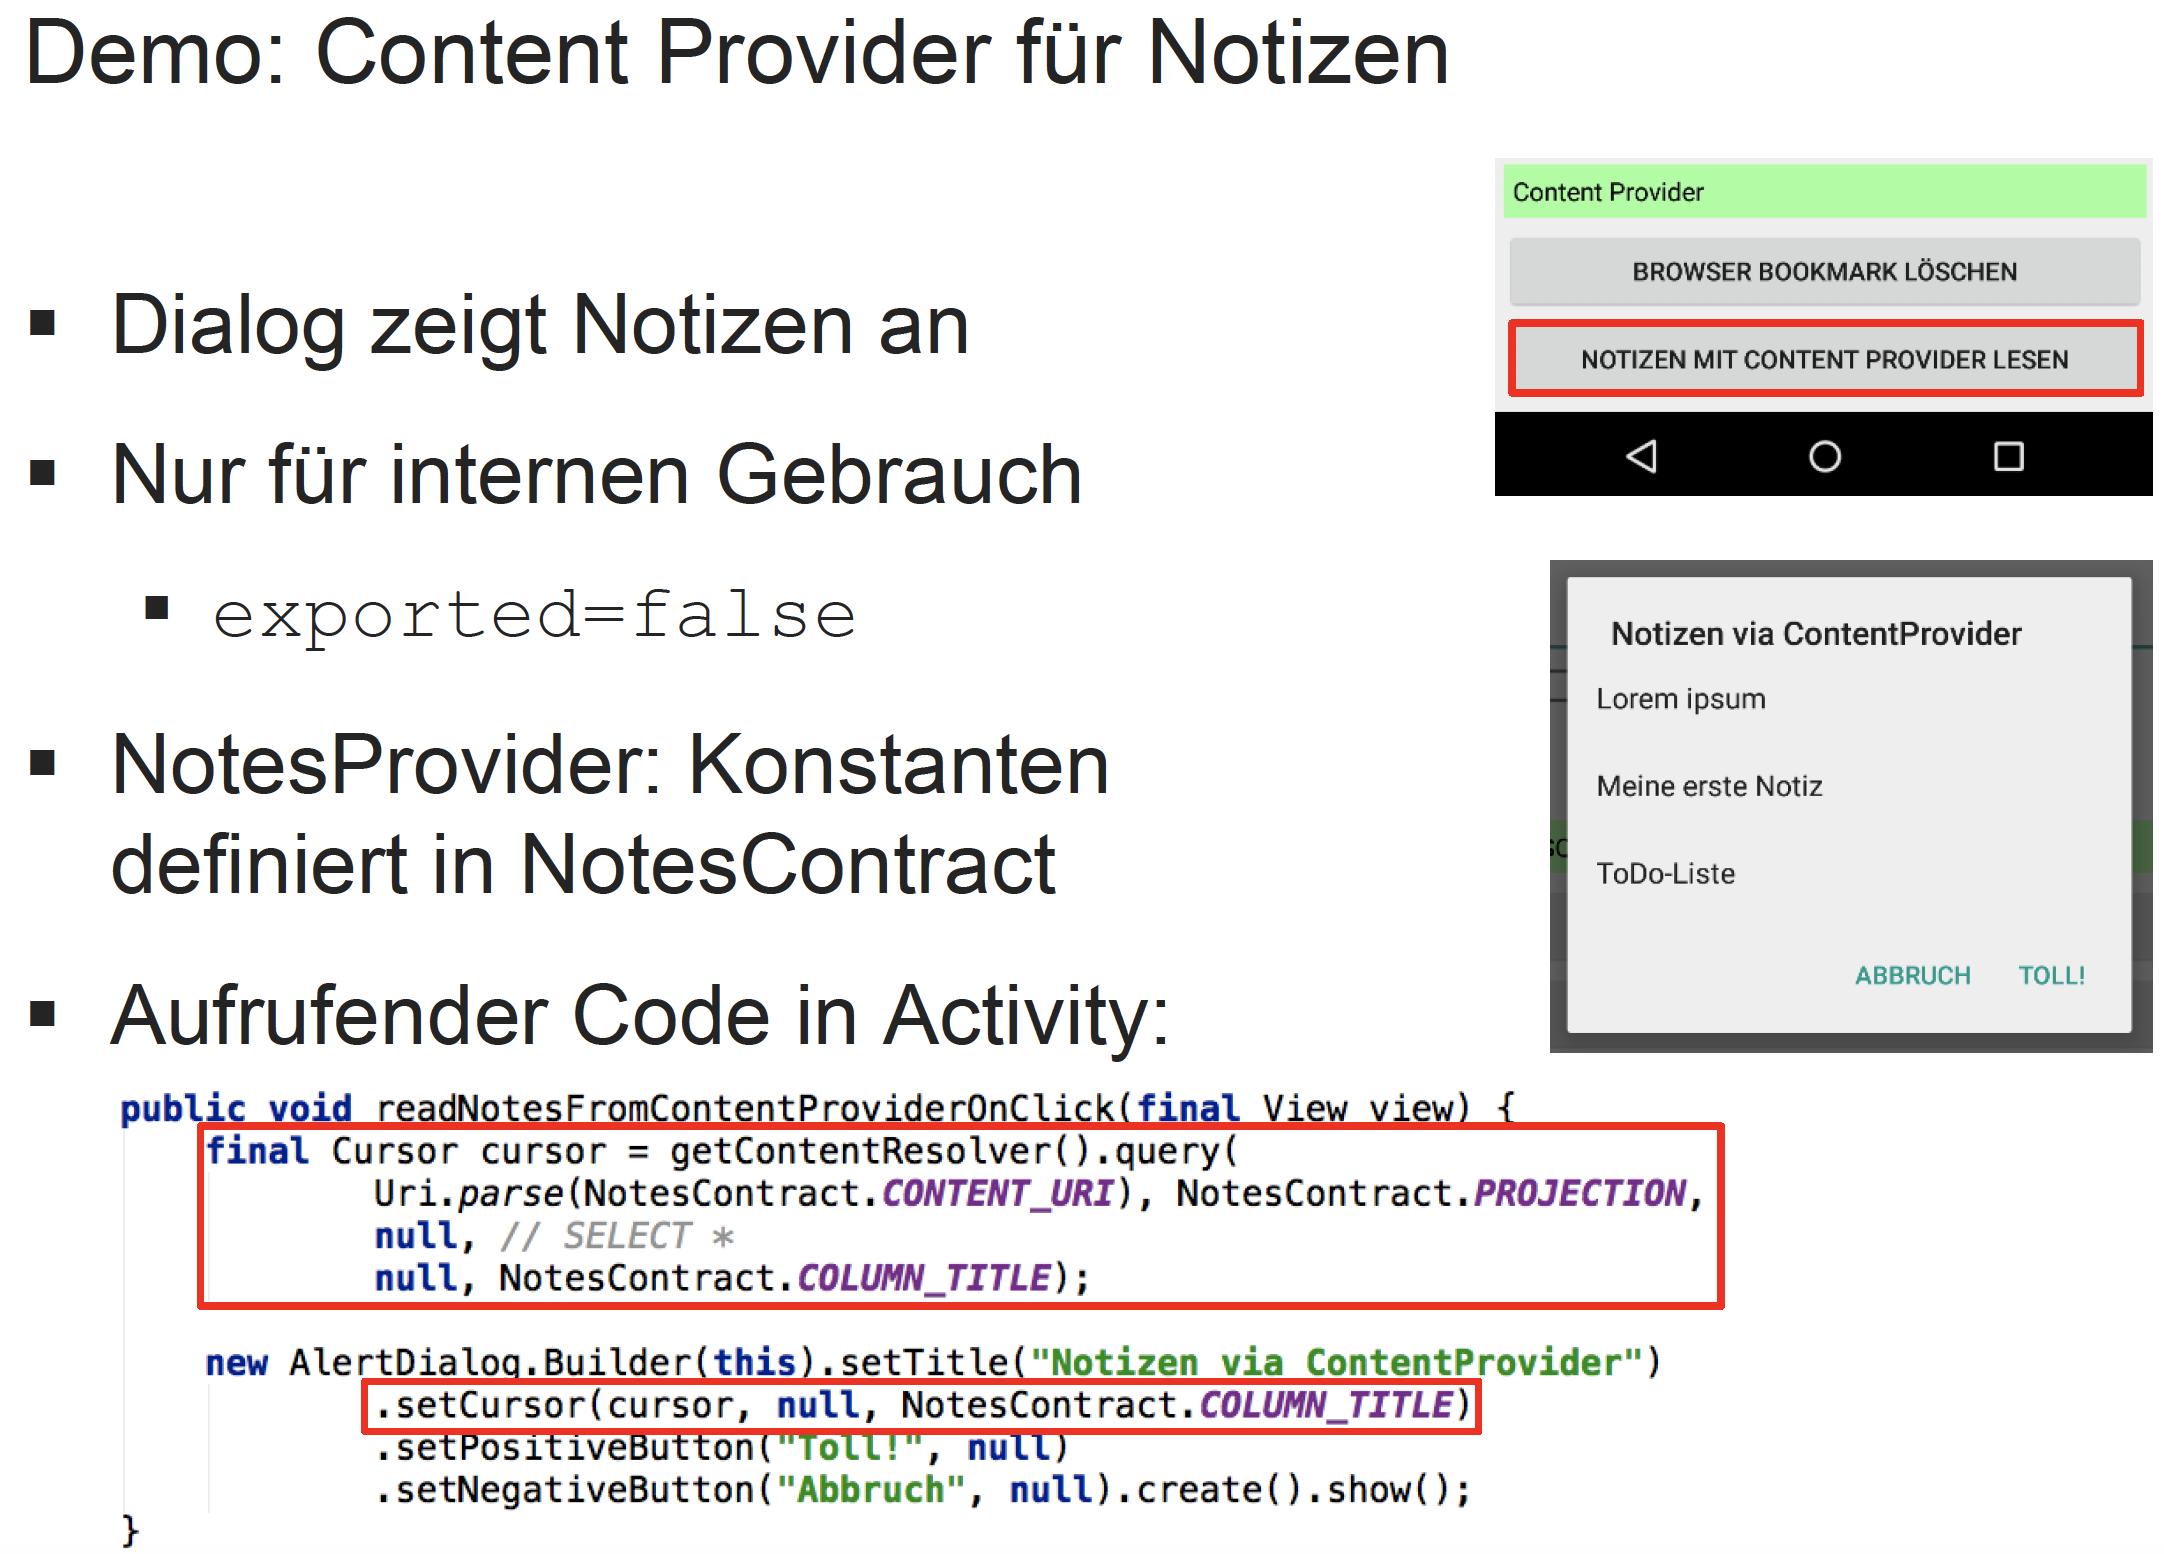
\includegraphics[width=.75\textwidth]{img/content_notes.png}
	\caption{Anwendungsbeispiel - Content Provider für Notizen}
\end{figure}

\section{Android 4 - Kommunikation \& Nebenläufigkeit}

\subsection{Nebenläufigkeit}

	\subsubsection{Android und der Main-Thread}

	\begin{itemize}
		\item Eine Applikation baut ihr UI nur auf einem Thread, dem \textbf{main-Thread} auf\\
		$\rightarrow$ blockiert man den main-Thread, friert das ganze UI ein
		\item UI-Komponenten sind nicht Thread-safe\\
		$\rightarrow$ UI-Zugriff nur aus main-Thread, sonst Exception
		\item Netzwerk- und andere Methoden können lange dauern und sind blockierend, werden diese auf dem main-Thread aufgerufen, wird er blockiert und es werden keine UI-Events mehr aufgerufen
	\end{itemize}

	\subsubsection{Android-Überwachung - ANR (Application Not Responding)}

		%TODO
	
\subsection{Nebenläufigkeit: AsyncTask}

		%TODO
	
\subsection{Nebenläufigkeit: Threads}

		%TODO

\subsection{(Backend-) Kommunikation über HTTP}

		%TODO
	
\subsection{JSON-Webservices mit Retrofit konsumieren}

		%TODO
	
\newpage
\section{Android 5 - Services \& Broadcast Receiver}

	%TODO

\newpage
\section{Android 6 - Intents, Fragments, App-Widgets}

	%TODO
	
\newpage
\section{Android 7 - Hybrid WebApp}

This was such a fucking shitshow, there's nothing to even talk about here.


\end{document}